\documentclass[12pt,a4paper,twoside]{article}
\usepackage[utf8]{inputenc}
\usepackage{setspace}
\usepackage{hyperref}
\usepackage[english]{babel}
\usepackage[nobiblatex]{xurl}
\usepackage{url}
\usepackage{graphicx}
\usepackage[left=3.5cm,right=2.5cm,top=2.5cm,bottom=2.5cm]{geometry}
\usepackage{fancyhdr}
\usepackage{float}

% Header and Footer
\pagestyle{fancy}
\fancyhead{} % clear header
\fancyfoot{}  % clear footer
\fancyfoot[LE,RO]{\thepage}
\renewcommand{\headrulewidth}{0pt}
\renewcommand{\footrulewidth}{0pt}

\renewcommand{\baselinestretch}{1.5} 

\begin{document}

\fontsize{14pt}{14pt}\selectfont
\begin{titlepage}
 \begin{center}
       Computer Science\\
       Akademia WSB\\
       Poland\\

      \vspace*{2cm}

      
\includegraphics[width=0.4\textwidth]{images-aws/university}

       \vspace*{3cm}
      
       \textbf{Subject: Corporate IT Infrastructure Project}
 
       \begin{center}
	\Large\textbf{Implementation of Github and Jenkins \\ as CI / CD}\\
       \end{center}

       \vspace{0.5cm}
        
            
       \vspace{1.5cm}


       \mbox{}\hfill \textbf{Lecturer:}  dr inż. Paweł Świtała

       {\raggedleft \textbf{Students:} Roman Tymochko, \par}
       {\raggedleft Dmitri Cerevatov,       \par}
       {\raggedleft Ioan Zîcu                    \par}


       \vfill
            

       \vspace{2cm}
     
       2020
            
   \end{center}
\end{titlepage}

\newpage

\fontsize{12pt}{12pt}\selectfont


\tableofcontents

~\newpage


\section{CI/CD Pipeline Introduction}


\subsection{What is a CI / CD pipeline?}


A \textbf{CI / CD pipeline} represents a tool that automates the software delivery process. The pipeline execute the custom scripts in order to build the project, run tests (CI), and deploys a new version of the application (CD) if there were not any fails.

The main benefits from the automated pipeline are the following:


\begin{itemize}
	\item Remove manual errors,
	\item Provide standardized feedback loops to developers,
	\item Enable fast product iterations.
\end{itemize}


\subsection{What do CI and CD means?}


\textbf{CI} stands for \textbf{Continuous Integration}, is a software development practice in which all developers merge code changes in a central repository multiple times a day.

Each change of the code triggers an automated build-and-test sequence for the given project and provide feedback to the developer who made the change. By default, the entire CI feedback loop run in maximum 10 minutes. But it can be adjusted if is needed.


\textbf{CD} stands for \textbf{Continuous Delivery}, which on top of Continuous Integration adds the practice of automating the entire software release process.

\textbf{Continuous Delivery} includes infrastructure provisioning and deployment, which may be manual and consist of multiple stages. All these processes are fully automated, each run is fully logged and available to the entire team.


\subsection{Elements of a CI/CD pipeline}


A CI/CD automate the specification of the steps that any developer needs to perform in order to deliver a new version of a software product. This automation allow developers to be more productive and not spend time by performing them manually.

The main stages through which goes the software release are \cite{ELEMENTS-CI/CD}:

\begin{itemize}
	\item \textbf{Source stage} - in the most common scenarios, the pipeline is triggered by a source code repository. A new change in the code triggers a notification (webhook) to the CI/CD tool, which runs the corresponding pipeline. Other common triggers include automatically scheduled or user-initialized workflows, or a results of other pipelines.

	\item \textbf{Build stage} - consist in combining the source code and its dependencies to build a runnable instance of the project the can be shipped to the end users. The projects written in languages like Java, C/C++, or Go need to be compiled, meanwhile Ruby, Python and JavaScript projects work without this step.

The cloud-native software is typically deployed with Docker, in which case the CI/CD pipeline will build the Docker container.

The most common errors related to this stage indicates fundamental problem in the project's configuration, and have a high priority.

	\item \textbf{Test stage} - here we run automated tests to validate our code's correctness and the behavior of our product. The test stage has the role of a safety net that prevents easily reproducible bugs from reaching the end-users.
The responsibility of writing tests falls on the developers. The best way to write automated tests is to do in parallel with the writing the new code in TDD (Test or Behavior Driven Development).

Depending of the size and complexity of the project, this phase can last from seconds to hours. Many large-scale projects run tests in multiple stages, starting with \textbf{smoke tests} that perform quick checks to \textbf{end-to-end integration tests} that test the entire system from the user's point of view. To reduce the test run time, an extensive test suite is parallelized.

Failure during the test stage exposes problems in the code that developers didn't foresee when writing the code. It is important that developers receive quick feedback at this stage, while the problem space is still fresh in their minds an they can maintain the state flow.

	\item \textbf{Deploy stage} - once we have a build of a runnable instance of our code that has passed the previous stages, the project is ready to deploy. There are usually multiple deploy environments like "beta" or "staging" environment which is used internally by the product team and a "production" environment for end-users.

The teams that use Agile model of development - guided by tests and real-time monitoring - usually deploy the work-in-progress manually to a staging environment for additional manual testing and review, and automatically deploy approved changes form the master branch to production.
\end{itemize}

The failure in each of the stages usually triggers a notification via email, Slack, etc, to let the responsible developer(s) to know about the causes. In case of the successful deployment in production, all team receives a notification.



~\newpage


\section{Jenkins CI/CD}


\textbf{Jenkins} is the leading open source, free to use (MIT License) automation server that provides hundreds of plugins to support building, deploying and automating any project. 

The Jenkins is written in Java and it was released in 2011 by the Kohsuke Kawaguchi. The source code is available on the GitHub Repository \url{https://github.com/jenkinsci/jenkins}.

Jenkins is a server-based system that runs in servlet containers such as Apache Tomcat. Jenkins allows Continuous Integration and Continuous Delivery of project, regardless of the platform, and can handle any kind of build or Continuous Integration. Using the variety of the available plugins, Jenkins can be integrated with many testing and deployment technologies.


The Jenkins usually will be installed on a server where the central build will take place. The following figure describe the simple Jenkins workflow.

\begin{figure}[H]
    \centering
        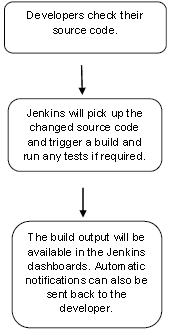
\includegraphics[width=4cm]{images-aws/jenkins_flowchart.png}
        \caption{Jenkins Flowchart \cite{JENKINS-FLOWCHART}}
\end{figure}


The hardware system requirements are: \textbf{JDK} - 1.5 or above, \textbf{Memory} - 2 GB RAM, 
 \textbf{Disk Space} - Since all builds will be stored on the Jenkins machines, it is recommended to ensure that there is available sufficient disk space, \textbf{Operating System Version} - Jenkins can be installed on Windows, Mac OS X, Linux, FreeBSD, OpenBSD, Gentoo; \textbf{Java Container} - The WAR file can be run in any container that supports Servlet 2.4/JSP 2.0 or later, for example Tomcat 5 \cite{JENKINS-FLOWCHART}.




~\newpage


\section{GitHub}


GitHub provides hosting for software development and Version Control using Git. It also offers distributed version control and source code management functionality of Git and other features like providing access control and several collaboration features such as bug tracking, feature requests, task management, continuous integration, and wikis for every project.


The basic services are offered free of charge. Free GitHub accounts are commonly used to host open-source projects. There are also commercial services dedicated to more advanced professionals and enterprises.


Github.com has the main purpose to facilitate the version control and issue tracking aspects of software development. Git allows pull requests to propose changes to the source code. Users with the ability to review the proposed changes can see a difference in the requested changes and approve them. This action is called "\textbf{committing}" and one instance of it is a "\textbf{commit}". All commits are saved there and can be reviewed later.
Labels, milestones, responsibility assignment, and a search engine are destined for issue tracking.


The other features of GitHub are:

\begin{itemize}
	\item \textbf{GitHub pages} - a static web hosting service, where users can host their project.
	\item \textbf{Gist} - allows hosting and share snippets of code.
	\item \textbf{Education program} called Github Student Developer Pack that gives students free access to popular tools and services. 
\end{itemize}








~\newpage


\section{Setup AWS EC2 Instance}




\begin{figure}[H]
    \centering
        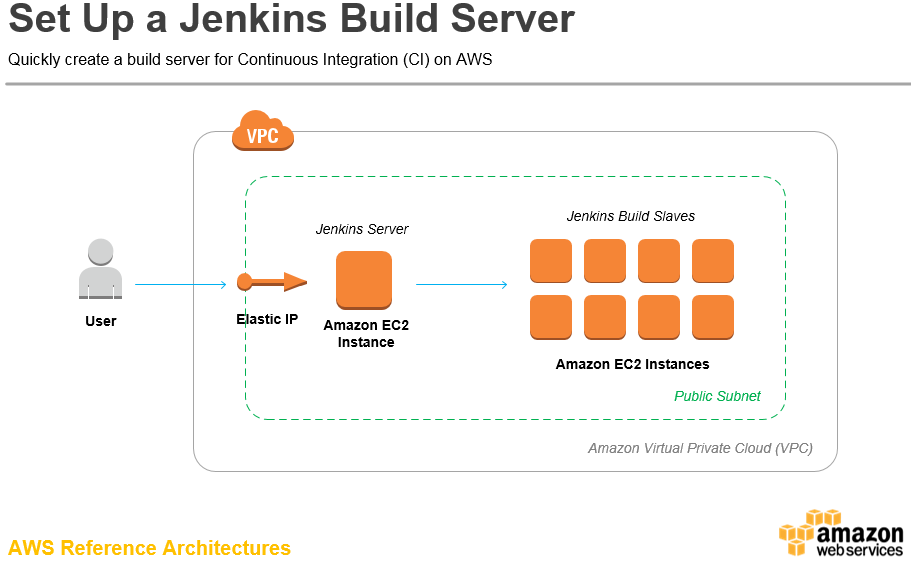
\includegraphics[width=15cm]{images-aws/aws-jenkins.png}
        \caption{AWS Jenkins Build Server Reference Architecture \cite{JENKINS-BUILD-SERVER}}
\end{figure}



\subsection{Create a Security Group for Amazon EC2 Instance}


We will create a security group and add the following rules:
\begin{itemize}
	\item Allow inbound HTTP access from anywhere
	\item Allow inbound SSH traffic from a specific computer's public IP address in order to connect to the instance
\end{itemize}


1. First of all we open the Amazon EC2 console \url{ https://console.aws.amazon.com/ec2/} 


2. In the navigation bar, we select \textbf{US West (Oregon)} region. This region use the Amazon EC2 console that is the newest version. If we select regions from Europe, then it will be available just Amazon VPC console, the older version.


\begin{figure}[H]
    \centering
        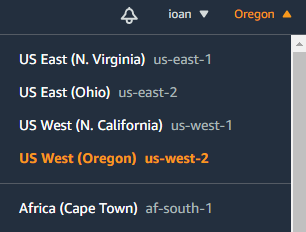
\includegraphics[width=7cm]{images-aws/1-aws-zone.png}
        \caption{AWS - select US West Zone}
\end{figure}


3. In the left-hand navigation bar, we choose the \textbf{Security Groups}, and then click on \textbf{Create Security Group}.


4. We name our Security Group \textbf{WebServerSecurityGroup} and select the VPC from the list.


5. In the \textbf{Inbound} tab, we add the following rules:
\begin{itemize}
	\item \textbf{HTTP} with source address 0.0.0.0/0 (basically open to any) and 46.187.163.63/32 (public IP address of the administrator)
	\item Open \textbf{port 8080} with source address 0.0.0.0/0 (basically open to any) and 46.187.163.63/32 (public IP address of the administrator)
	\item \textbf{SSH}   source address 46.187.163.63/32 - just administrator to be able to access the instance via SSH.
	\item \textbf{HTTPS} with source address 0.0.0.0/0 (basically open to any) and 46.187.163.63/32 (public IP address of the administrator)
\end{itemize}


\begin{figure}[H]
    \centering
        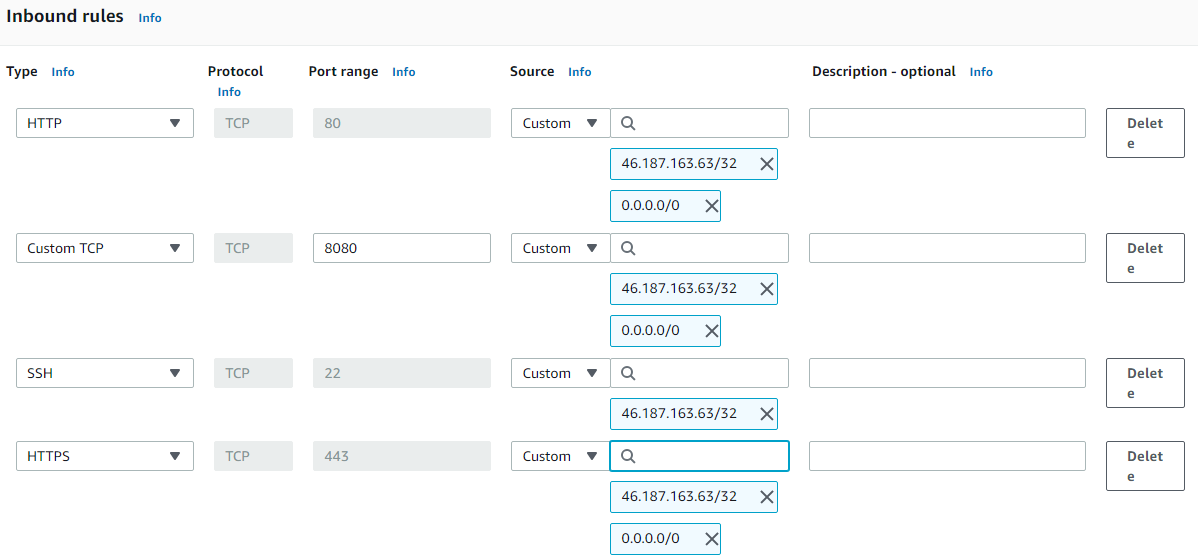
\includegraphics[width=15cm]{images-aws/2-inbound-rules.png}
        \caption{Setup rules for inbound traffic}
\end{figure}


6. Then we click \textbf{Create}.


\begin{figure}[H]
    \centering
        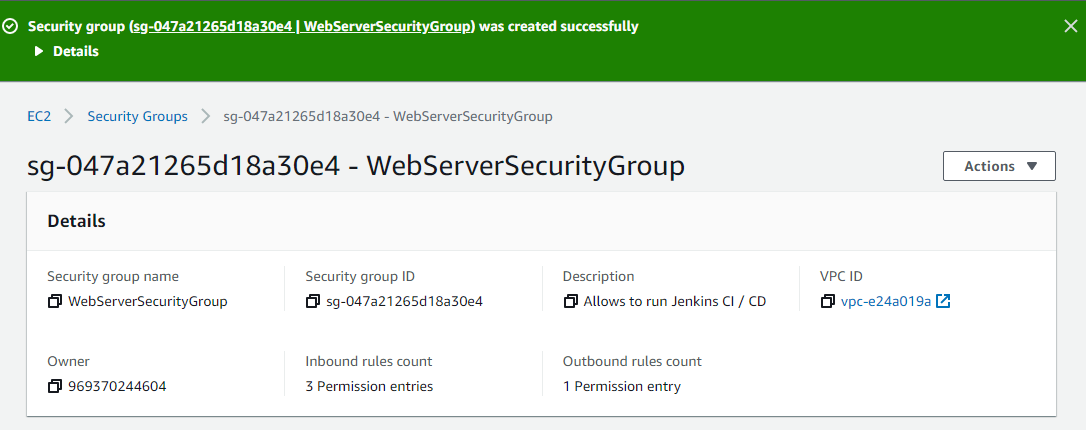
\includegraphics[width=15cm]{images-aws/3-create-sg-created.png}
        \caption{Security Group was successfully created}
\end{figure}


~\newpage

\subsection{Launch the Amazon EC2 Instance}


1. In the left-hand navigation bar of the Amazon EC2 console, we select \textbf{Instances}, and click \textbf{Launch Instance}.


\begin{figure}[H]
    \centering
        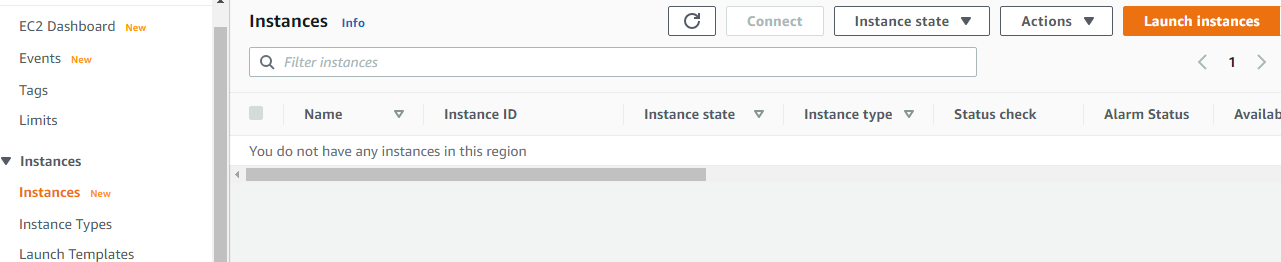
\includegraphics[width=15cm]{images-aws/4-instances.png}
        \caption{Navigate to Instances Menu}
\end{figure}


2. On the \textbf{Choose an Amazon Machine Image page}, we select an Amazon Linux AMI with the HVM virtualization type.


\begin{figure}[H]
    \centering
        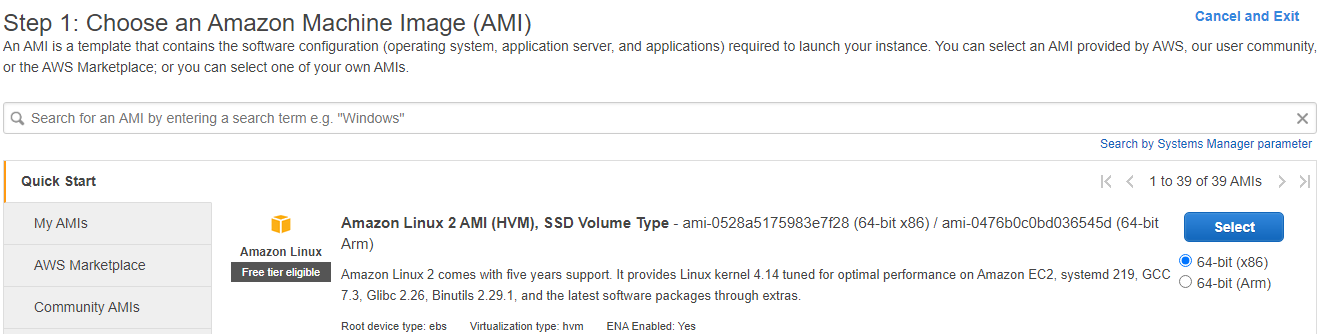
\includegraphics[width=15cm]{images-aws/5-amazon-linux.png}
        \caption{Choose Amazon Linux 2 AMI Virtual Machine}
\end{figure}


3. On the \textbf{Choose an Instance Type} page, the \textbf{t2.micro} instance is selected by default. We keep this instance type to stay within the free tier.


4. Then we click \textbf{Next: Configure Instance Details}


\begin{figure}[H]
    \centering
        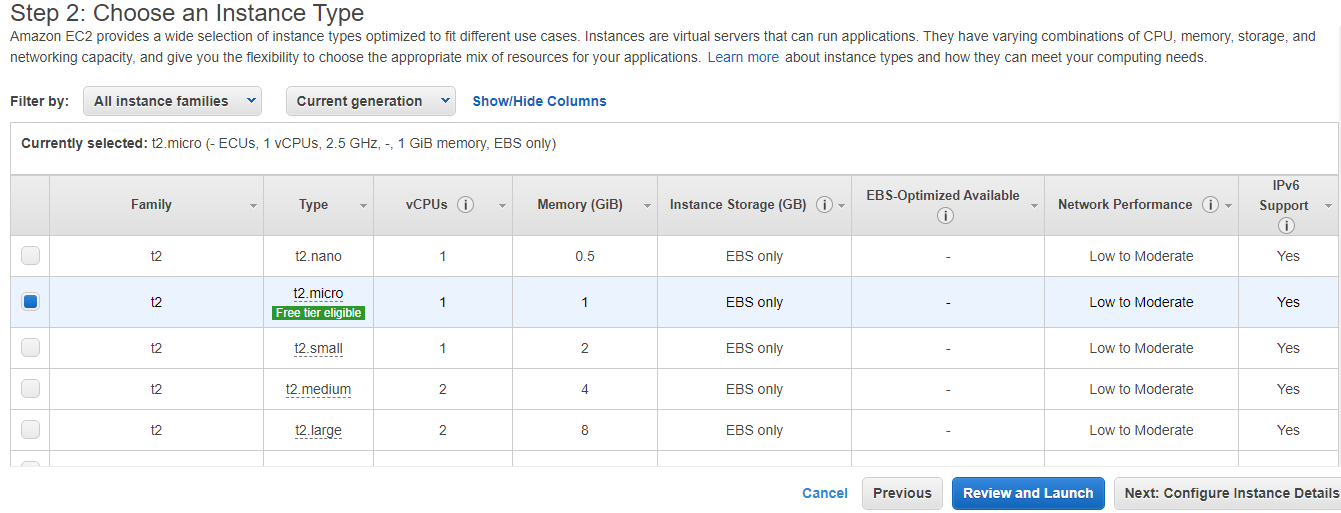
\includegraphics[width=15cm]{images-aws/6-instance-type.png}
        \caption{Choose t2.micro Instance, Free Tier}
\end{figure}


5. On the \textbf{Configure Instance Details} page we do the following:


\begin{itemize}
	\item From the \textbf{Network} we choose the VPC, and from \textbf{Subnet} we choose the \textbf{public} subnet.
	\item We ensure that in the \textbf{Auto-assign Public IP} the option \textbf{Enable} is selected. Otherwise the instance will not
get a public IP address or a public DNS name.
	\item Click \textbf{Review and Launch}.
\end{itemize}


\begin{figure}[H]
    \centering
        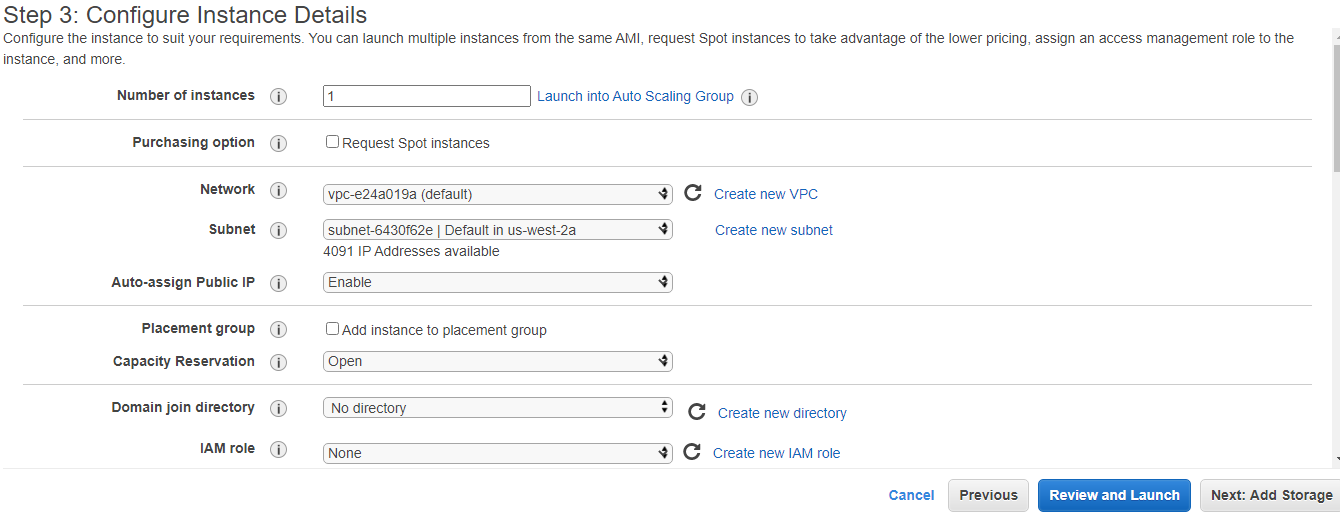
\includegraphics[width=15cm]{images-aws/7-config-instance-details.png}
        \caption{Configure Instance Details}
\end{figure}


6. On the \textbf{Review and Launch} page we click \textbf{Edit security groups}.


7. On the \textbf{Configure Security Group} page we select the \textbf{WebServerSecurity Group} that we created and then click \textbf{Review and Launch}.


\begin{figure}[H]
    \centering
        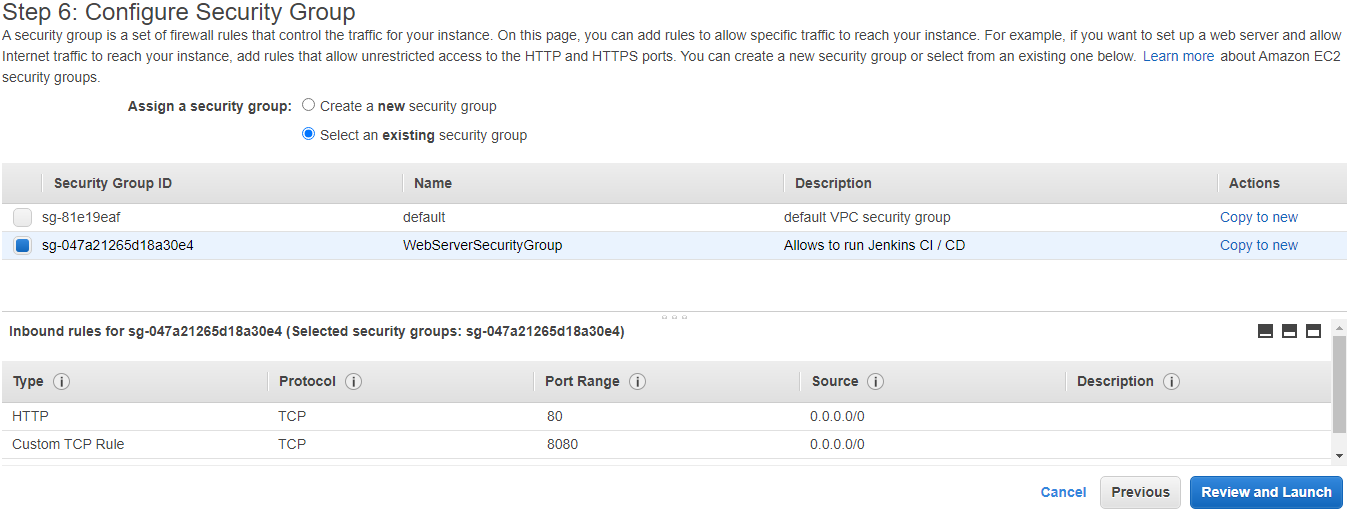
\includegraphics[width=15cm]{images-aws/8-config-sec-group.png}
        \caption{Configure Security Group}
\end{figure}


8. On the \textbf{Review Instance Launch} page, we click \textbf{Launch}.


\begin{figure}[H]
    \centering
        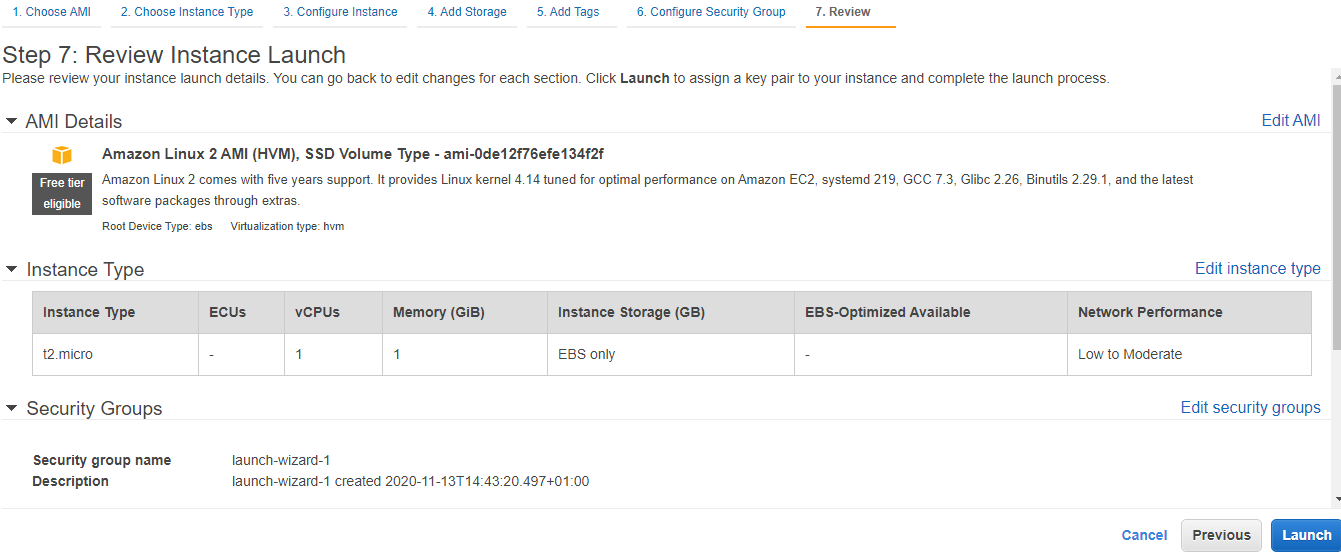
\includegraphics[width=15cm]{images-aws/9-review-instance-launch.png}
        \caption{Review Instance Launch}
\end{figure}


9. Next, in the \textbf{Select an existing key pair or create a new key pair} dialog box, we select \textbf{Create a new key pair} and enter the name. After creating the key in .pem format we will be able to access the instance via SSH.


\begin{figure}[H]
    \centering
        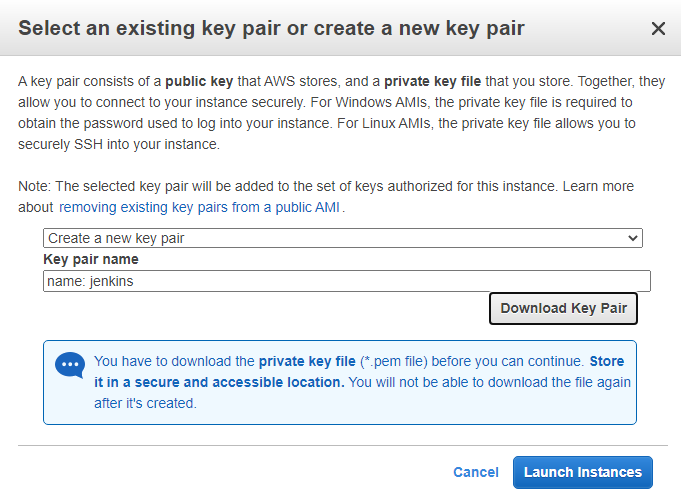
\includegraphics[width=8cm]{images-aws/10-key-pair.png}
        \caption{Create a new key pair}
\end{figure}


10. Click on the \textbf{Launch Instances} button.


\begin{figure}[H]
    \centering
        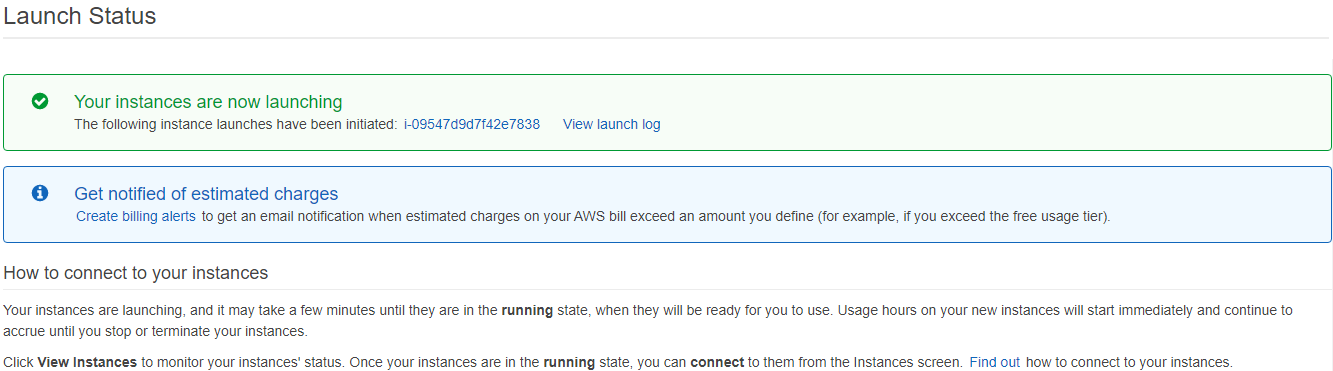
\includegraphics[width=15cm]{images-aws/11-launch-status.png}
        \caption{Launch Status}
\end{figure}


We make sure that the instance is up and running.


\begin{figure}[H]
    \centering
        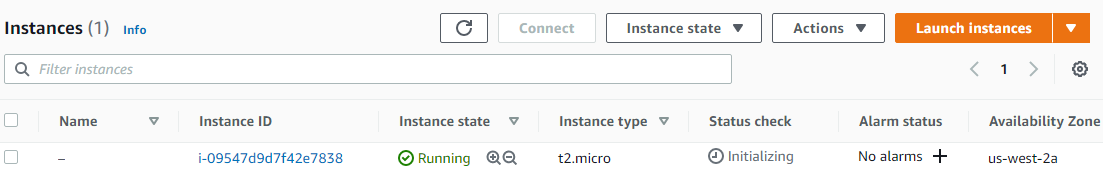
\includegraphics[width=15cm]{images-aws/12-running-instance.png}
        \caption{Verify Running Instance}
\end{figure}



~\newpage


\section{Install and Configure Jenkins}


\subsection{Connect to the EC2 Instance using SSH}


After the instance was launched, we can connect to it and use it via SSH bash shell. For this purpose we will use the \textbf{Git Bash} tool.


1. From \textbf{Git Bash} we use the \textbf{ssh} command to connect to the instance. We specify the private key (.pem) file and the ec2-user@public\_dns\_name.

\begin{verbatim}
ssh -i namejenkins.pem 
ec2-user@ec2-52-12-213-243.us-west-2.compute.amazonaws.com
\end{verbatim}

\begin{figure}[H]
    \centering
        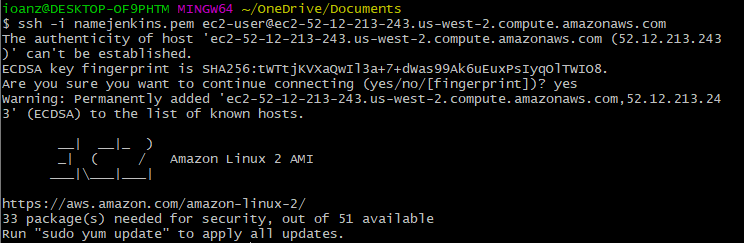
\includegraphics[width=15cm]{images-aws/13-ssh-connect.png}
        \caption{SSH into Amazon Linux 2 AMI}
\end{figure}


\subsection{Download and Install Jenkins}


1. We first ensure that software packages are up to date.


\begin{verbatim}
sudo yum update -y
\end{verbatim}


\begin{figure}[H]
    \centering
        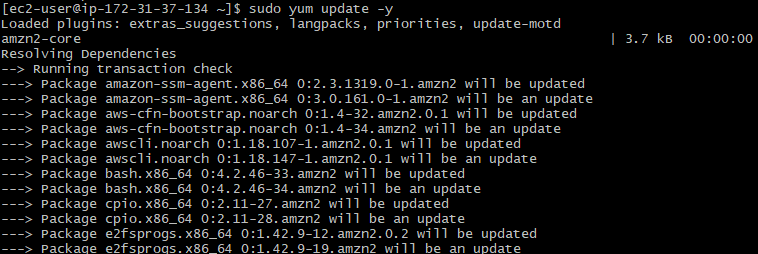
\includegraphics[width=15cm]{images-aws/14-yum-update.png}
        \caption{Update packages}
\end{figure}


2. Jenkins will require Java JDK, so we install it on the EC2 instance.


\begin{verbatim}
sudo yum install java-1.8.0-openjdk
\end{verbatim}


\begin{figure}[H]
    \centering
        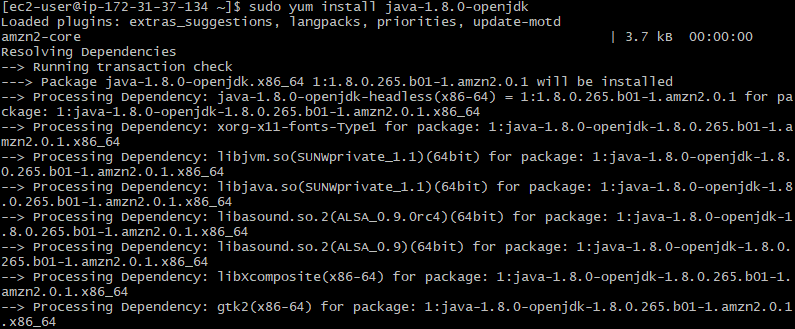
\includegraphics[width=15cm]{images-aws/15-install-java.png}
        \caption{Install Java Open JKD}
\end{figure}


3. We add Jenkins repository using the following command:


\begin{verbatim}
sudo wget -O
/etc/yum.repos.d/jenkins.repo http://pkg.jenkins-
ci.org/redhat/jenkins.repo
\end{verbatim}


\begin{figure}[H]
    \centering
        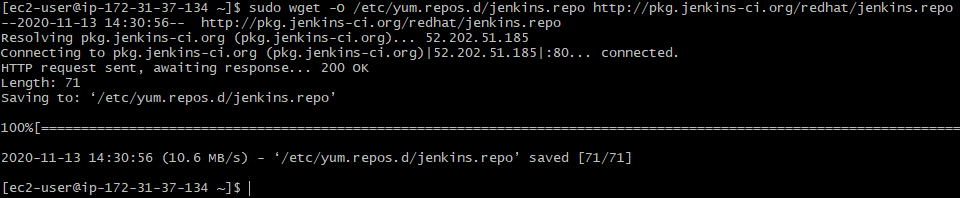
\includegraphics[width=15cm]{images-aws/16-download-jenkins.png}
        \caption{Add Jenkins repository}
\end{figure}


4. Import a key file from Jenkins-CI to enable installation from the package:


\begin{verbatim}
sudo rpm --import
https://pkg.jenkins.io/redhat/jenkins.io.key
\end{verbatim}


\begin{figure}[H]
    \centering
        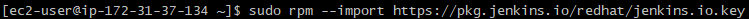
\includegraphics[width=15cm]{images-aws/17-import-jenkins-keys.png}
        \caption{Import Jenkins official keys to enable installation from the package}
\end{figure}


5. Install Jenkins:


\begin{verbatim}
sudo yum install jenkins -y
\end{verbatim}


\begin{figure}[H]
    \centering
        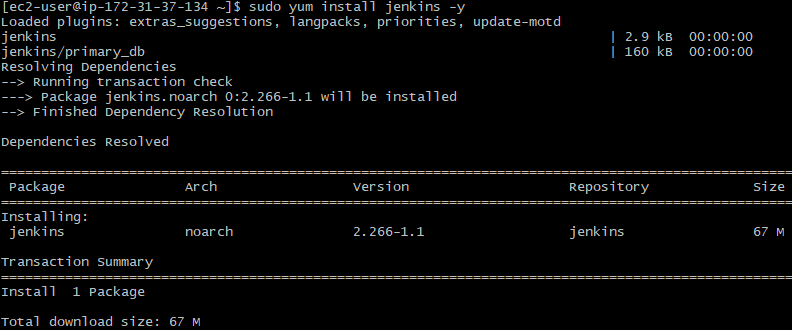
\includegraphics[width=15cm]{images-aws/18-install-jenkins.png}
        \caption{Install Jenkins}
\end{figure}


6. Start Jenkins as a service:


\begin{verbatim}
sudo service jenkins start
\end{verbatim}


\begin{figure}[H]
    \centering
        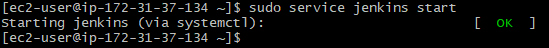
\includegraphics[width=11cm]{images-aws/19-start-jenkins.png}
        \caption{Start Jenkins Service}
\end{figure}



\newpage

\subsection{Configure Jenkins}


Jenkins is now available and running on the EC2 instance. To configure Jenkins we:


1. Connect to the \url{http://ec2-52-12-213-243.us-west-2.compute.amazonaws.com:8080/} using Chrome browser.
Then we will be able to access the Jenkins management interface.


\begin{figure}[H]
    \centering
        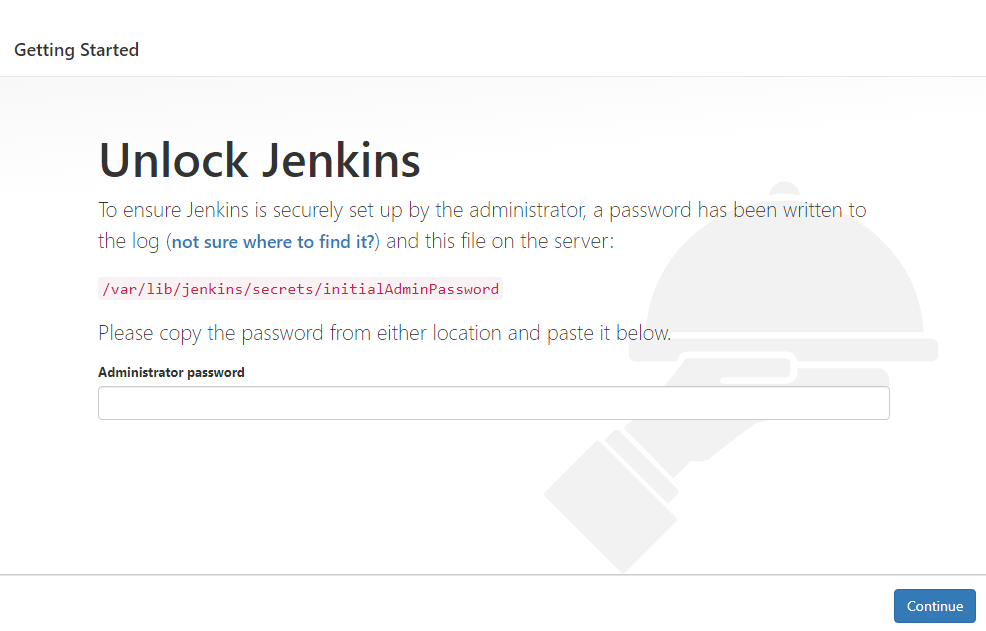
\includegraphics[width=15cm]{images-aws/20-unlock-jenkins.png}
        \caption{Unlock Jenkins}
\end{figure}


2. We print on the console the initial admin password found in

 \textbf{/var/lib/jenkins/secrets/initialAdminPassword}, 

using the following command:


\begin{verbatim}
sudo cat
/var/lib/jenkins/secrets/initialAdminPassword
\end{verbatim}


\begin{figure}[H]
    \centering
        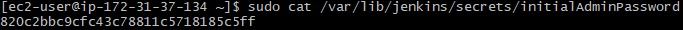
\includegraphics[width=13cm]{images-aws/21-get-jenkins-admin-pass.png}
        \caption{Get initial Admin Password}
\end{figure}


3. The Jenkins installation script directs to the \textbf{Customize Jenkins} pages. We click on the  \textbf{Install suggested plugins}.


\begin{figure}[H]
    \centering
        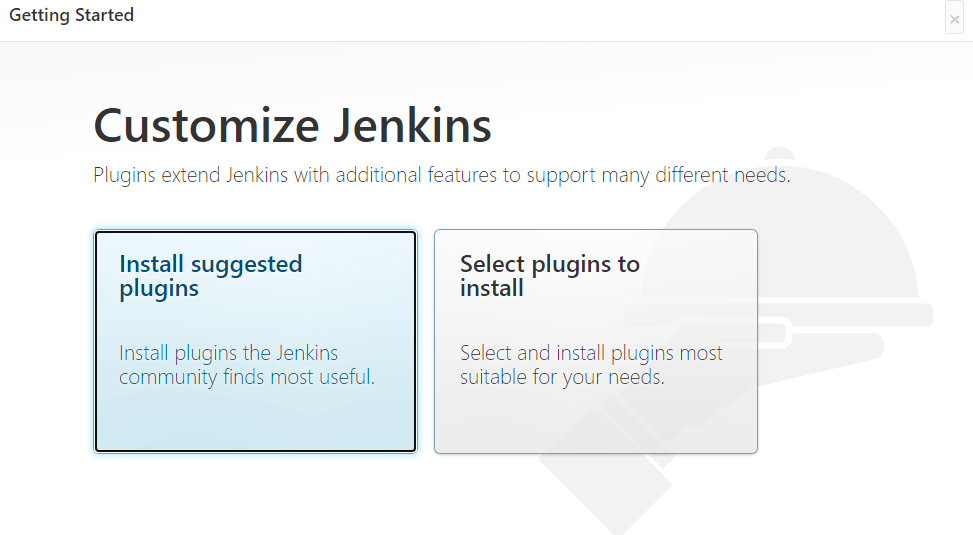
\includegraphics[width=15cm]{images-aws/22-jenkins-select-plugin.png}
        \caption{Customize Jenkins}
\end{figure}


4. We search for the \textbf{GitHub} plugin, select it and install.


\begin{figure}[H]
    \centering
        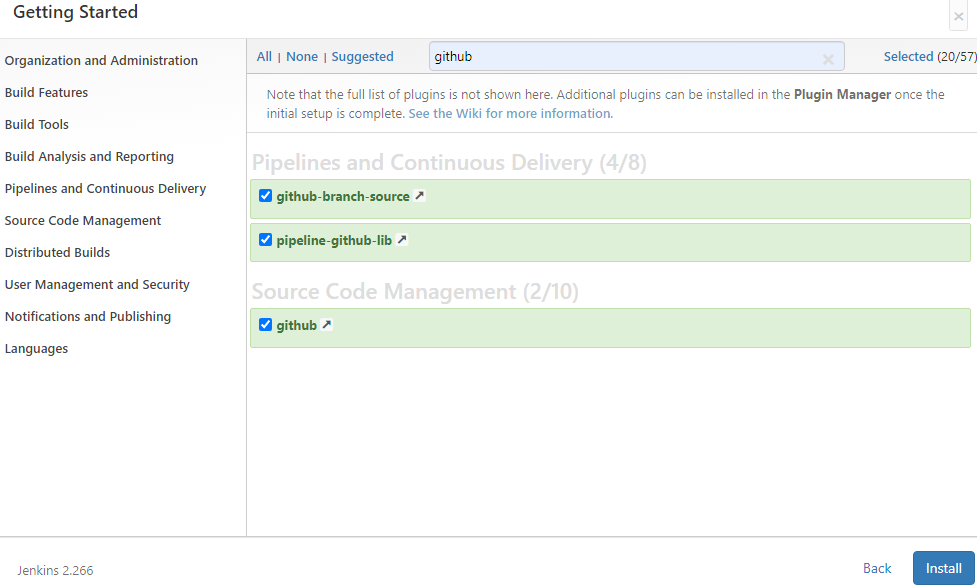
\includegraphics[width=15cm]{images-aws/23-jenkins-select-github-plugin.png}
        \caption{Select GitHub Plugin to be Installed}
\end{figure}


~\newline


5. Once the installations is completed, we enter Administrator Credentials and click \textbf{Save and Continue}.


\begin{figure}[H]
    \centering
        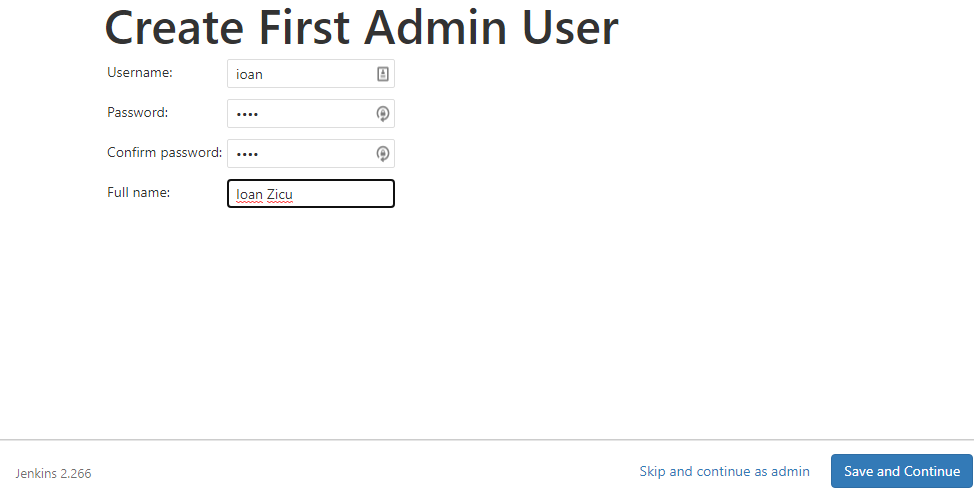
\includegraphics[width=15cm]{images-aws/24-jenkins-admin-user.png}
        \caption{Create First Admin User}
\end{figure}


6. Next window is \textbf{Instance Configuration} where we can see the Jenkins URL. We click \textbf{Save and Finish}.


\begin{figure}[H]
    \centering
        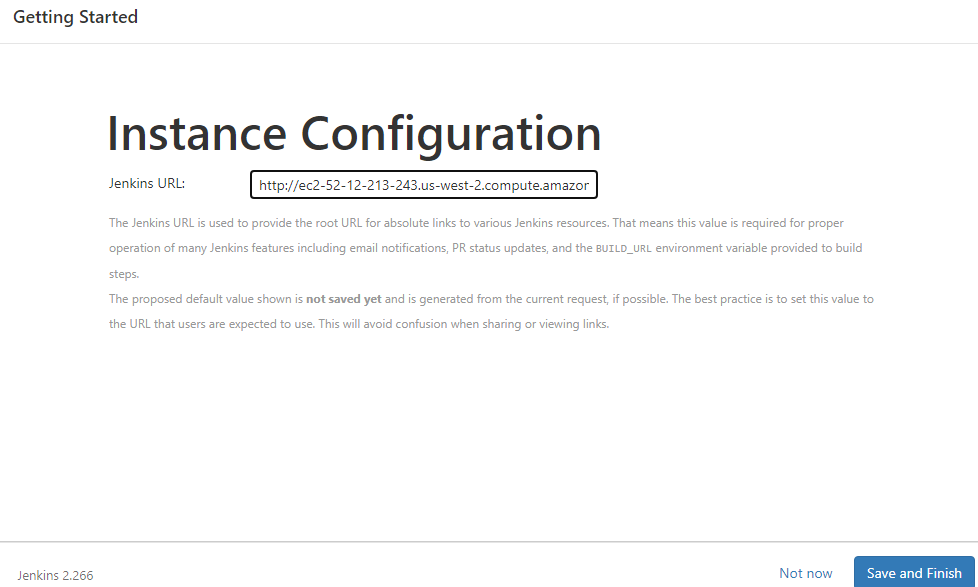
\includegraphics[width=15cm]{images-aws/25-jenkins-conf.png}
        \caption{Instance Configuration}
\end{figure}


At this moment we have completed the Jenkins setup.


\begin{figure}[H]
    \centering
        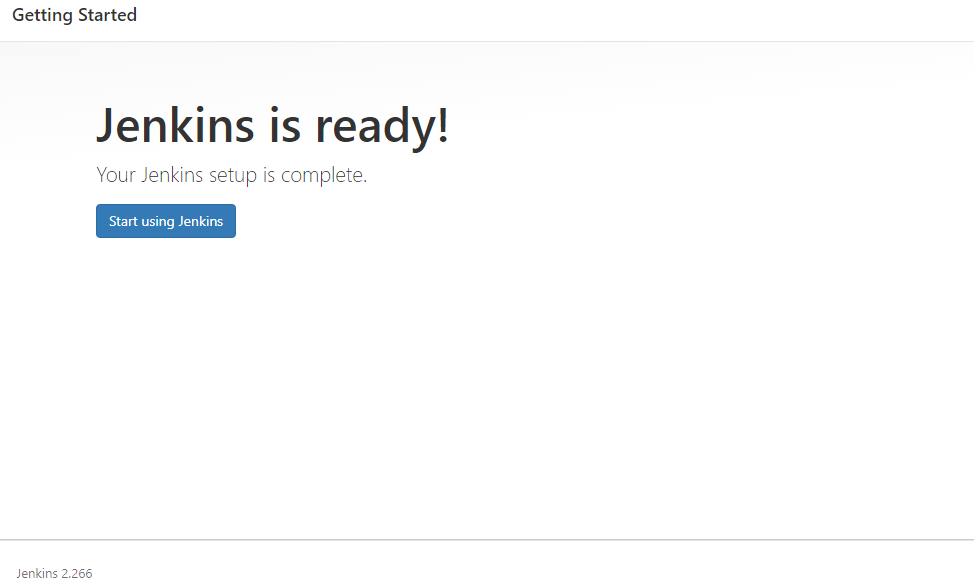
\includegraphics[width=15cm]{images-aws/26-jenkins-ready.png}
        \caption{Jenkins is Ready}
\end{figure}


~\newpage


\section{Setup a Jenkins Job for Our Project}


In Jenkins, the software projects are built in the separate Jobs. 
But before proceeding to the creating of a Jenkins Job, we have to install some prerequisites. 


\begin{itemize}
	\item First we have to install \textbf{Git} on the EC2, to allow to get the project's files from the GitHub repository.

	\item Second is specific for this concrete project, we need to have Golang programming language for the build environment, so we will install the \textbf{Go Plugin}. In different project it can be required different programming languages like Java, Python, C\#, etc, so this is depending of the specific project.
\end{itemize}


\subsection{Install Git on EC2}


We want to setup the \textbf{Source Code Repository} to have access to the project code. So we enter the \textbf{Repository URL}.
At this moment, we receive error because we haven't installed \textbf{Git} on our  Amazon Linux EC2 Instance.


In the bash shell that is connected to the EC2 instance to install \textbf{git} we enter the following command:


\begin{verbatim}
sudo yum install git -y
\end{verbatim}


\begin{figure}[H]
    \centering
        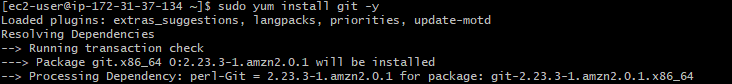
\includegraphics[width=15cm]{images-aws/27-jenkins-install-git.png}
        \caption{Install Git}
\end{figure}


To setup git executable file into the Jenkins Configuration Menu we identify it's location with \textbf{which} command.


\begin{verbatim}
which git
\end{verbatim}


\begin{figure}[H]
    \centering
        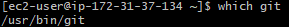
\includegraphics[width=6cm]{images-aws/28-jenkins-git-on-local.png}
        \caption{Get Git location}
\end{figure}


After installation of \textbf{Git} on the EC2 instance we go to \textbf{Dashboard} -> \textbf{Global Tool Configuration}, scroll to \textbf{Git} section and paste the path in the \textbf{Path to Git executable} field and we click \textbf{Save} button.


\begin{figure}[H]
    \centering
        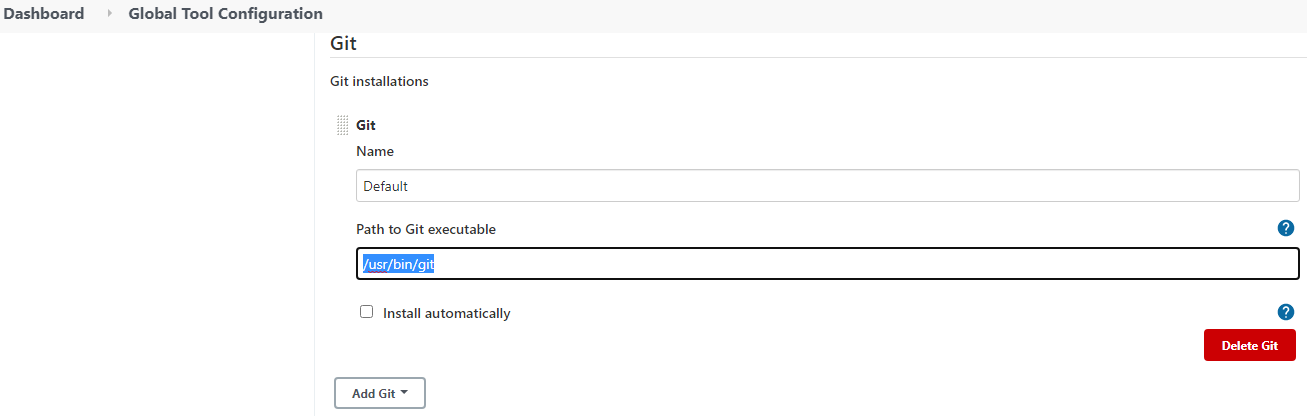
\includegraphics[width=15cm]{images-aws/29-jenkins-git-set-path.png}
        \caption{Setup Git path to the executable}
\end{figure}



~\newpage


\subsection{Setup Go Plugin for Build Environment}


Because our project is written in Go and requires Golang Environment, we install the \textbf{Go} plugin, that will help us in setting up the language version for the specific build.

We navigate into \textbf{Dashboard} - \textbf{Plugin Manager} and search for the \textbf{Go} plugin, select is and the click the button \textbf{Install without restart} button.


\begin{figure}[h!]
    \centering
        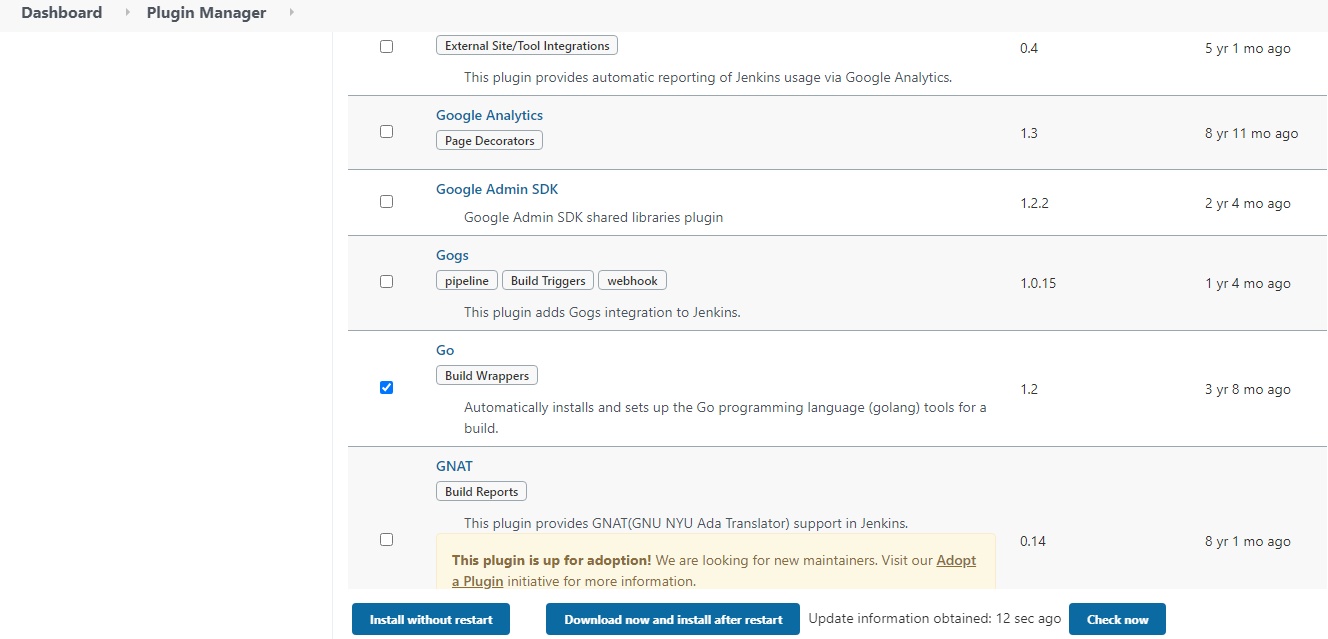
\includegraphics[width=15cm]{images-aws/30-go-plugin.png}
        \caption{Setup Plugin for Golang Programming Language}
\end{figure}


Next, we navigate to \textbf{Dashboard} - \textbf{Global Tool Configuration}, check the \textbf{Install automatically} checkbox, select version of Go \textbf{1.15} and click on \textbf{Save} button.


\begin{figure}[h!]
    \centering
        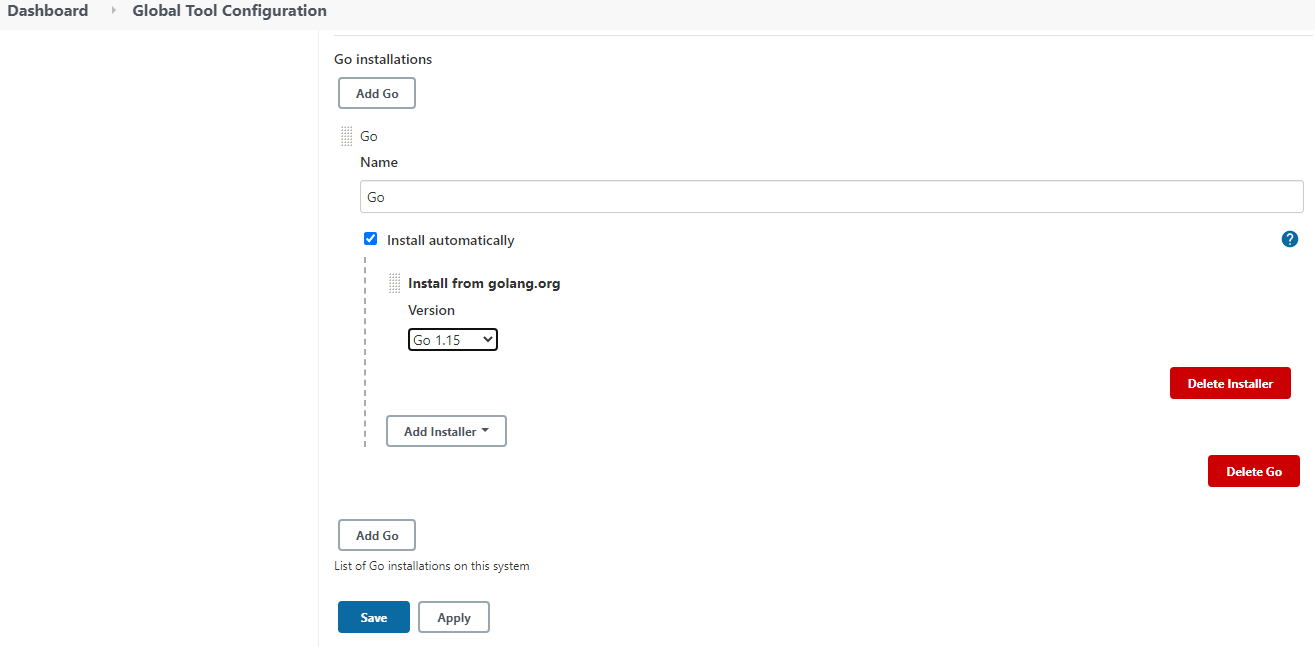
\includegraphics[width=15cm]{images-aws/31-go-global-tool.png}
        \caption{Configure Golang Version}
\end{figure}



~\newpage


\subsection{Create Jenkins Job}


In order to create a Job for our project we click on 
\textbf{Create a job} item.


\begin{figure}[H]
    \centering
        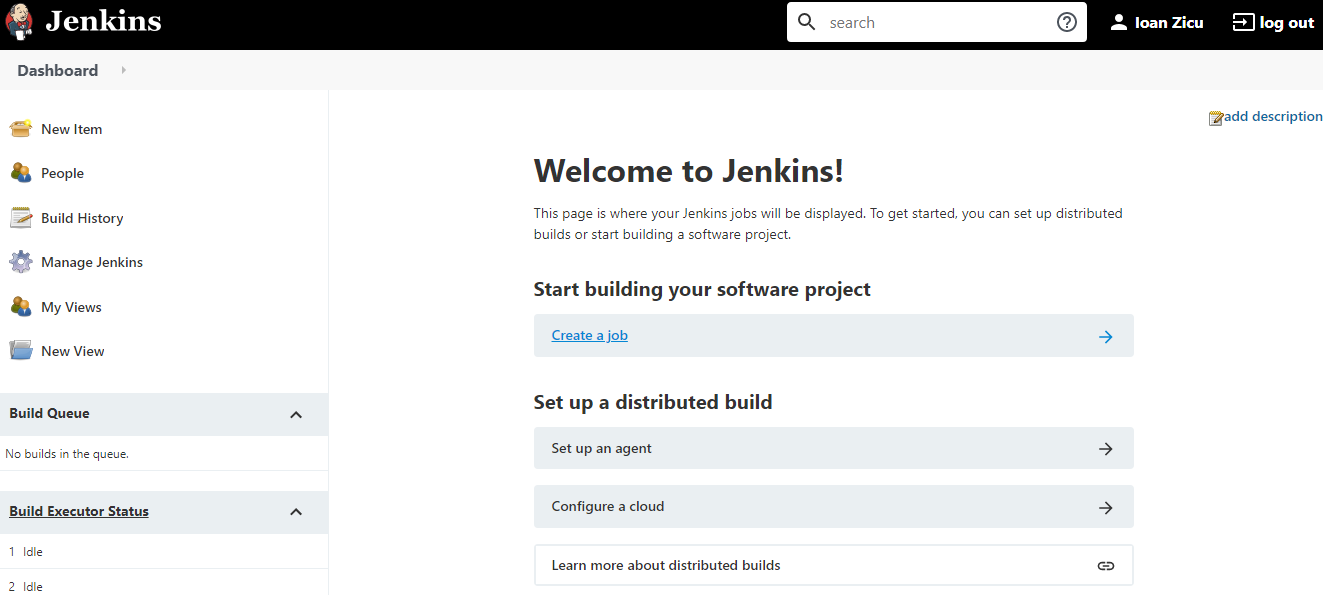
\includegraphics[width=15cm]{images-aws/32-jenkins-create-job.png}
        \caption{Create a Jenkins Job}
\end{figure}


Next, we enter the item name for the project \textbf{RouteFinderApp} and select the \textbf{Freestyle project} option and click \textbf{OK}.


\begin{figure}[H]
    \centering
        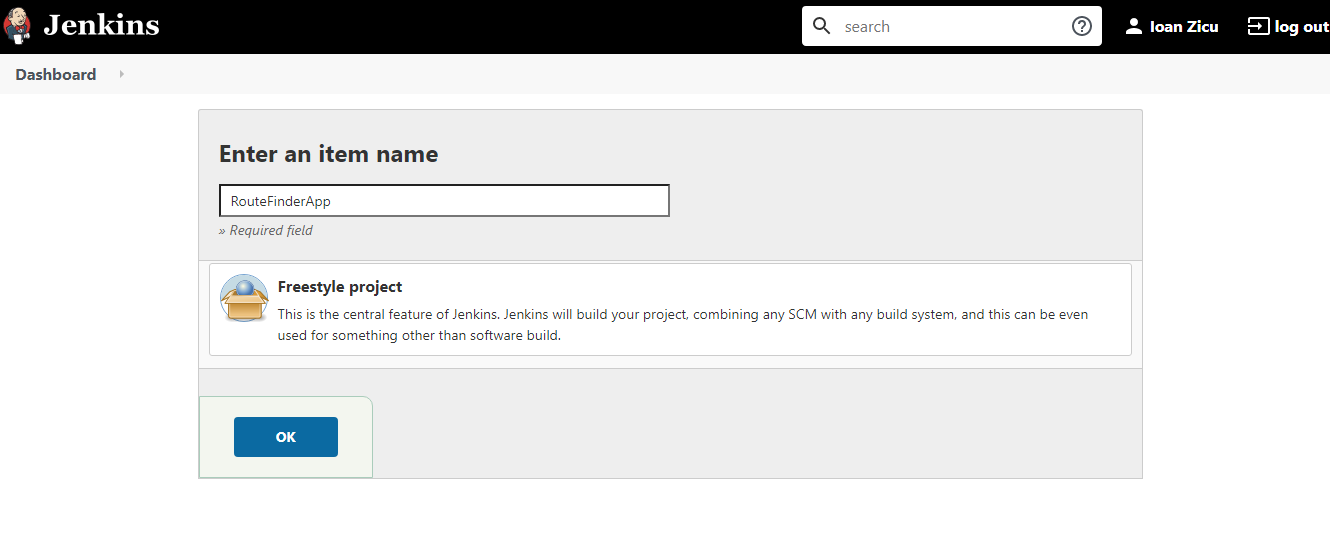
\includegraphics[width=15cm]{images-aws/33-jenkins-set-project-name.png}
        \caption{Enter the project name}
\end{figure}


In the \textbf{Source Code Management} tab, we select \textbf{Git} and insert the \textbf{Repository URL}.


\begin{figure}[H]
    \centering
        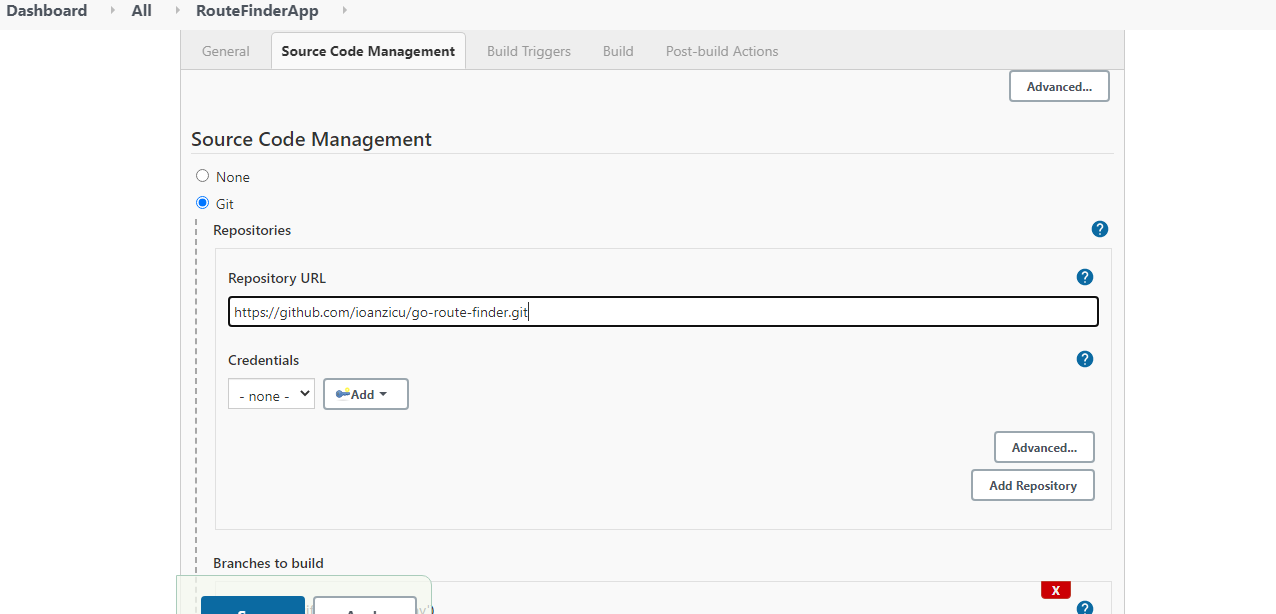
\includegraphics[width=15cm]{images-aws/34-jenkins-setup-repo-no-error.png}
        \caption{Setup GitHub Repository}
\end{figure}


In the \textbf{Build Triggers} menu, in the \textbf{React build Action} dropdown, we select and click on \textbf{Execute shell}.


\begin{figure}[H]
    \centering
        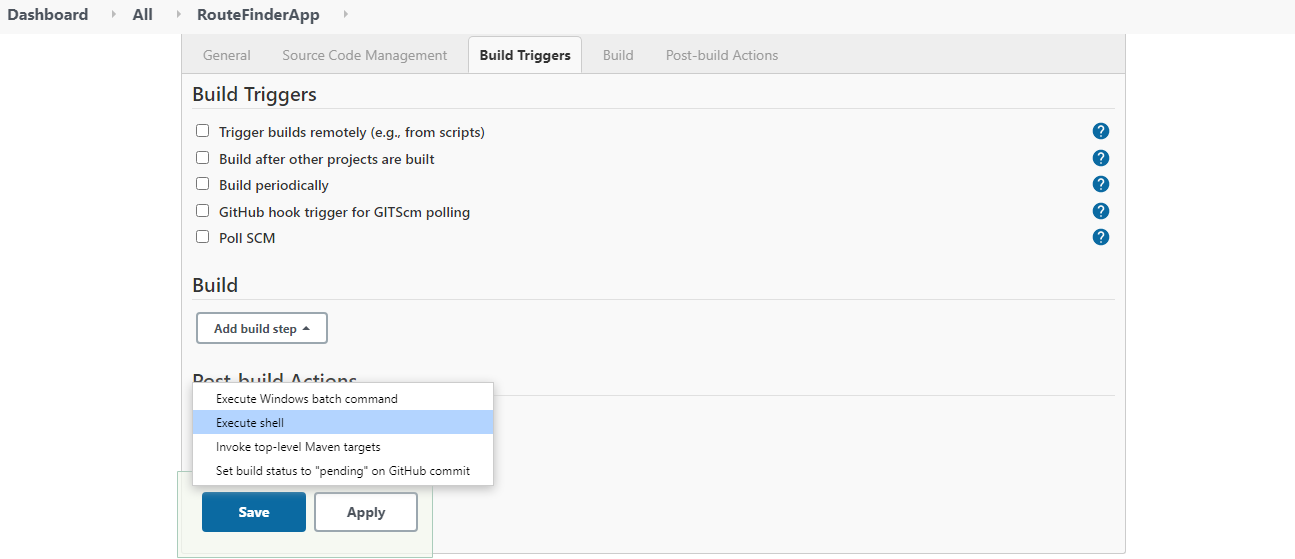
\includegraphics[width=15cm]{images-aws/35-jenkins-build-setup.png}
        \caption{Setup Build Triggers}
\end{figure}


In \textbf{Build Environment} tab, we select \textbf{Set up Go programming language tools}, then select \textbf{Go version} that we have setup before (1.15).
In \textbf{Build} subsection, we write commands for the \textbf{Executive shell}, mainly to:


\begin{itemize}
	\item Enable Environment Variables for Golang, 
	\item Download Project Dependencies,
	\item Build the Project,
	\item Run Unit Tests.
\end{itemize}


Then we click \textbf{Save} button.


\begin{figure}[H]
    \centering
        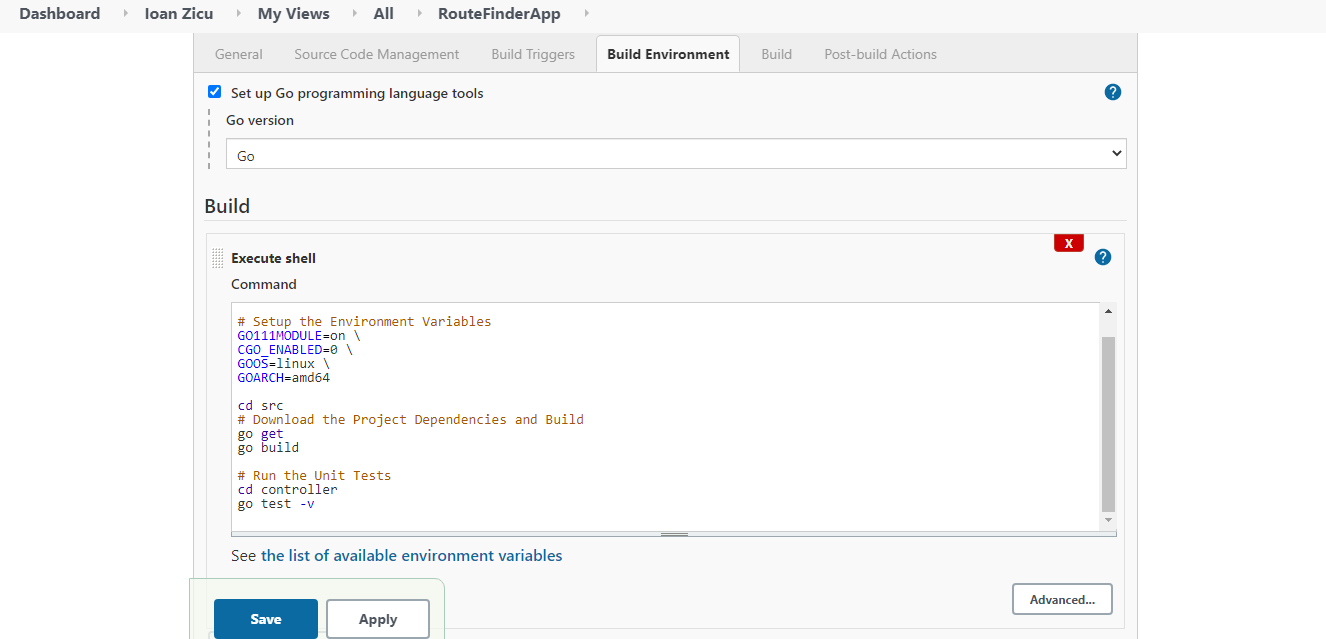
\includegraphics[width=15cm]{images-aws/36-project-build-env-golang-.png}
        \caption{Setup Script for Build Environment}
\end{figure}


We have successfully created a Jenkins Job, and Jenkins have access to the project source code from the GitHub.


\begin{figure}[H]
    \centering
        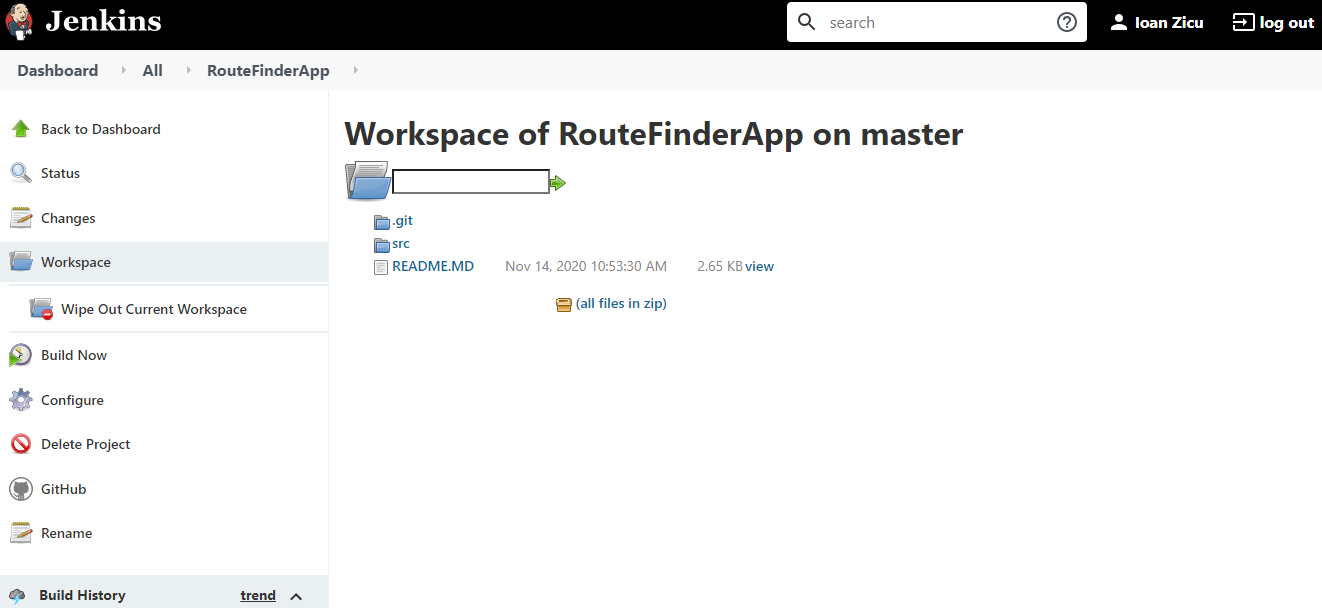
\includegraphics[width=15cm]{images-aws/37-project-workspace-git.png}
        \caption{Project Work Space}
\end{figure}


In left-hand side bar, we click on \textbf{Build Now} to manually test if the project is building in the Jenkins Workspace. Then, we navigate to the build's \textbf{Console Output} and see the job logs.


\begin{figure}[H]
    \centering
        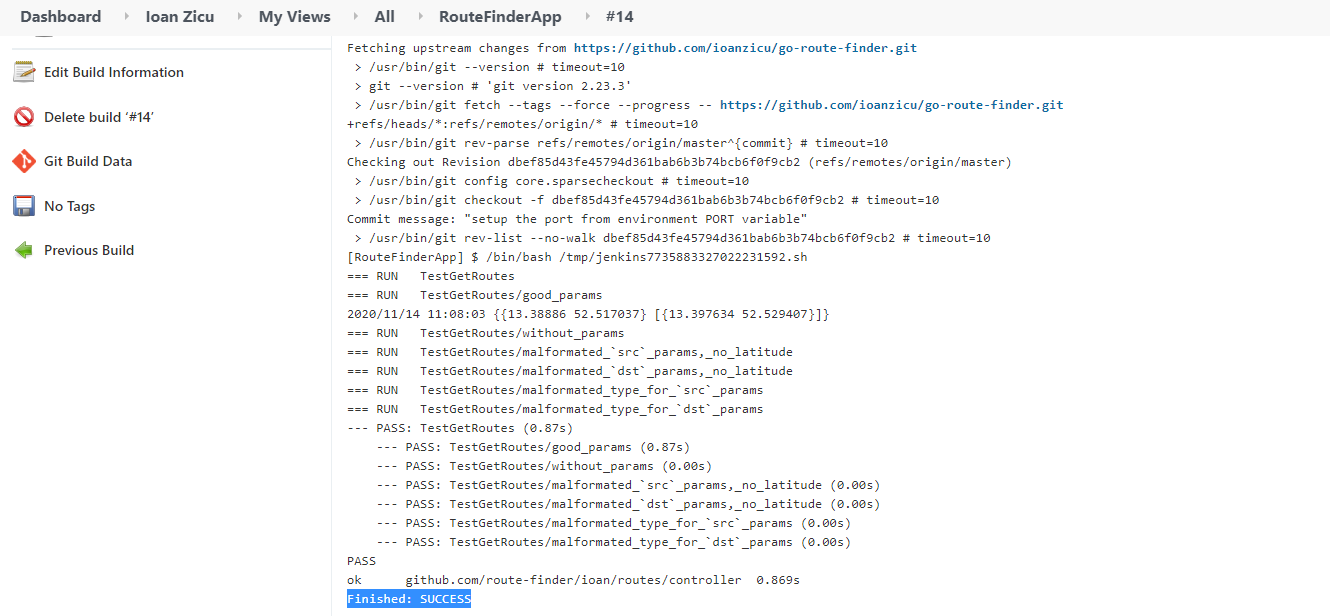
\includegraphics[width=15cm]{images-aws/38-test-build.png}
        \caption{Run the Project Build}
\end{figure}


On \textbf{Dashboard} page, we see the \textbf{RouteFinderApp} job listed with the information about the Last Success, Last Fail and Duration of the Last build.


\begin{figure}[H]
    \centering
        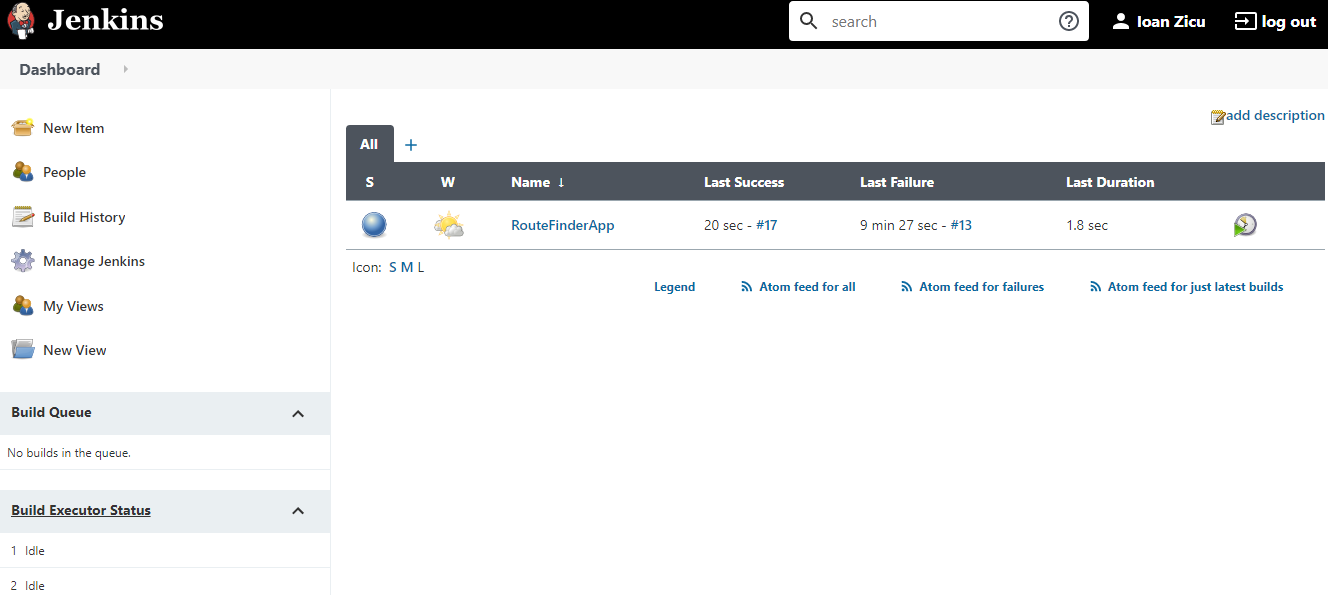
\includegraphics[width=15cm]{images-aws/39-test-build-success.png}
        \caption{Project Status}
\end{figure}



~\newpage


\subsection{Setup webhook on the GitHub repository}


In this chapter, we want to setup a webhook in the GitHub repository in order to automatically trigger Jenkins Job Build at each \textbf{Push} and \textbf{Pull Request} event. 

This is a most common scenario of the integration of Jenkins with GitHub in the Software Development Life-cycle.


On GitHub repository page, we click on the \textbf{Settings} button.


\begin{figure}[H]
    \centering
        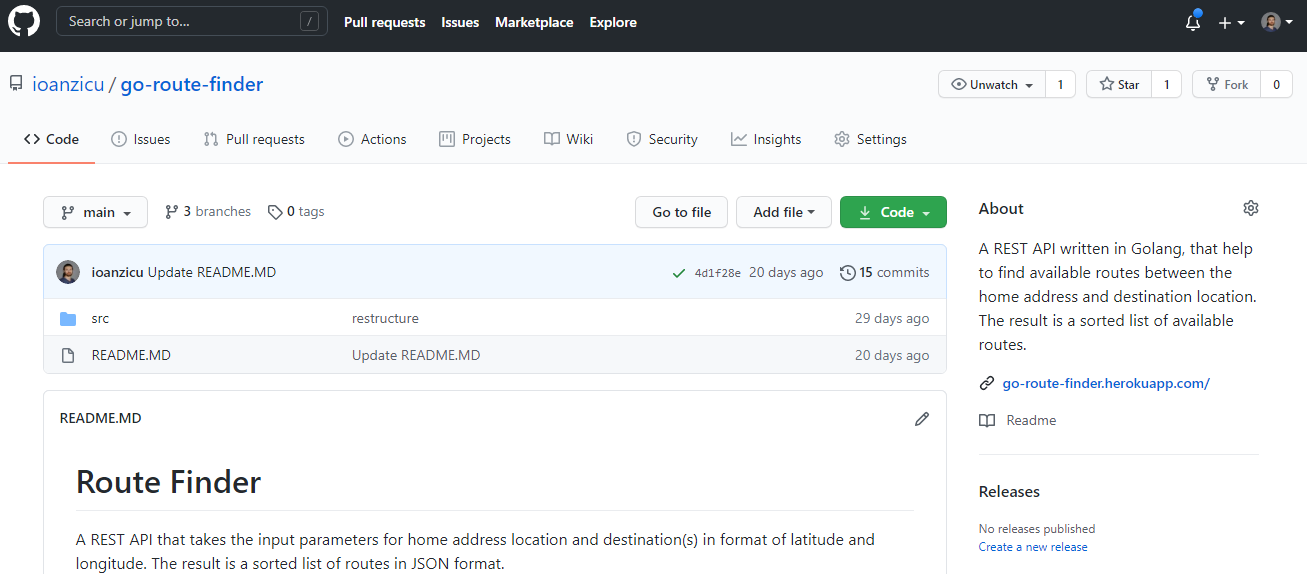
\includegraphics[width=15cm]{images-aws/40-github-project.png}
        \caption{RouteFinder Application GitHub Repository}
\end{figure}


From the left-hand side bar, we click on \textbf{Webhooks}. We can see that on this repository there is already one webook. In the right hand-side, we click on \textbf{Add webhook} button.


\begin{figure}[H]
    \centering
        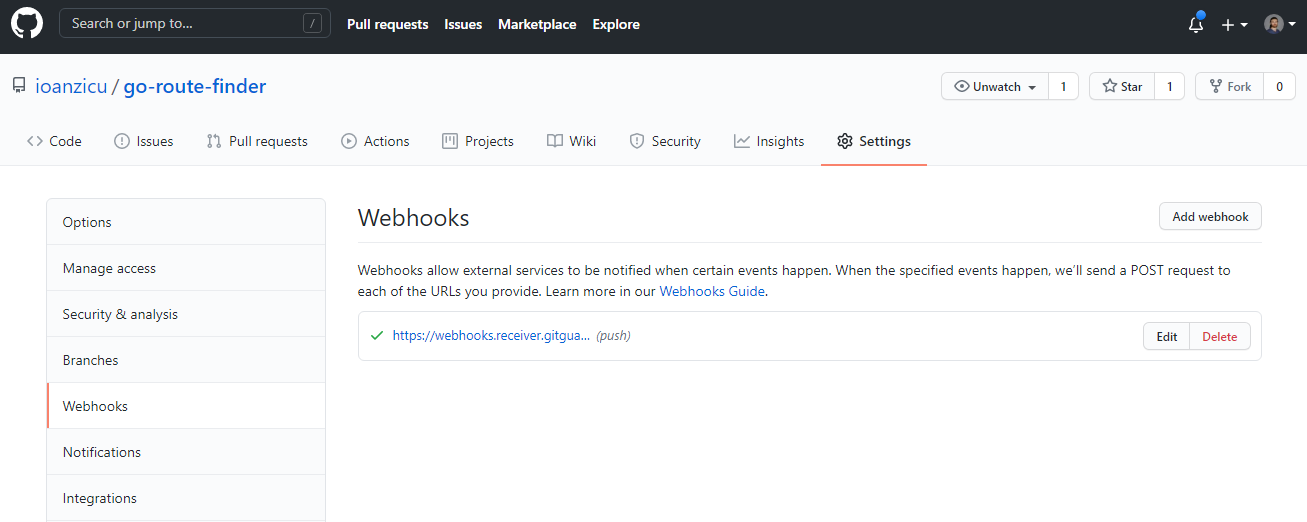
\includegraphics[width=15cm]{images-aws/41-web-hook.png}
        \caption{Check Webhooks}
\end{figure}


On \textbf{Webhooks / Add webhook} subpage we paste the \textbf{Payload URL}  with port 8080 at the end, which in fact is the URL to the Jenkins located in the EC2 instance.


\textbf{Content Type} is \textbf{application/json} and we specify that we want to \textbf{Select individual events}.


\begin{figure}[H]
    \centering
        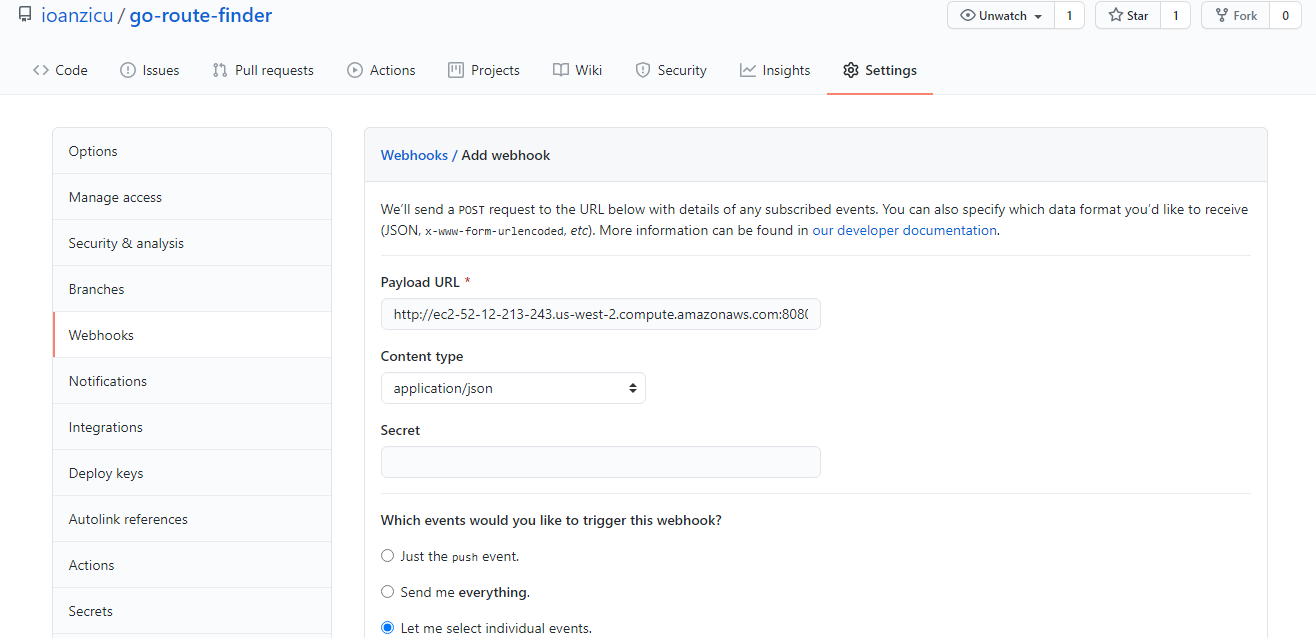
\includegraphics[width=15cm]{images-aws/42-web-hook-setup.png}
        \caption{Add new Webhook to trigger Jenkins Build}
\end{figure}


From the list of events, we select \textbf{Pull request} and \textbf{Pushes}.


\begin{figure}[H]
    \centering
        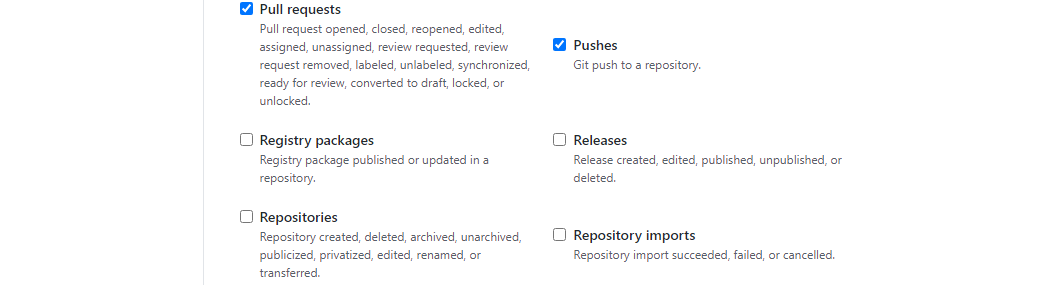
\includegraphics[width=13cm]{images-aws/43-web-hook-setup-pull.png}
        \caption{Trigger Jenkins Build on Push and Pull Request}
\end{figure}

 We check the \textbf{Active} checkbox at the bottom of the page. Then we click on \textbf{Add webhook}.

\begin{figure}[H]
    \centering
        
\includegraphics[width=13cm]{images-aws/44-web-hook-setup-activate.png}
        \caption{Activate Event Details}
\end{figure}


We have successfully created a new Webhook. But we can see that there is a black dot in  front of it, which means this webhook was not triggered yet.


\begin{figure}[H]
    \centering
        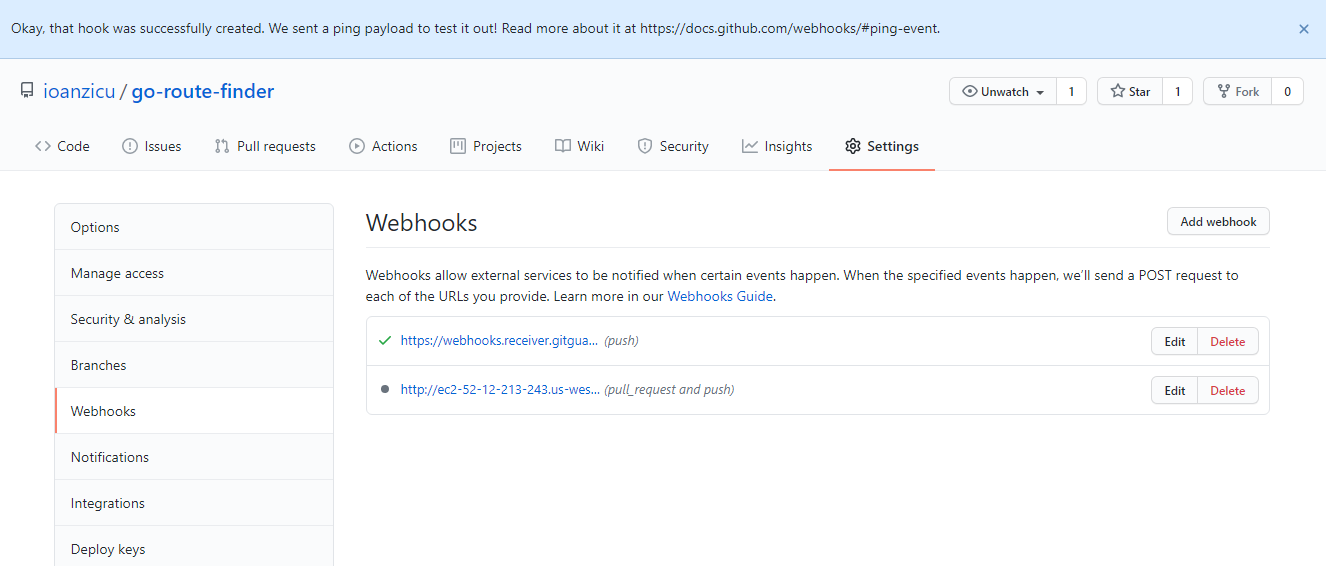
\includegraphics[width=15cm]{images-aws/45-web-hook-created.png}
        \caption{Webhook successfully created}
\end{figure}


Next, we have to edit Configuration for our project build on Jenkins. In the \textbf{Dashboard} we select the \textbf{RouteFinderApp} project, then on the left hand-side click on \textbf{Configure}, select \textbf{Build Triggers} tab and check option \textbf{GitHub hook trigger for GITScm polling}. After we click \textbf{Save} button.


\begin{figure}[H]
    \centering
        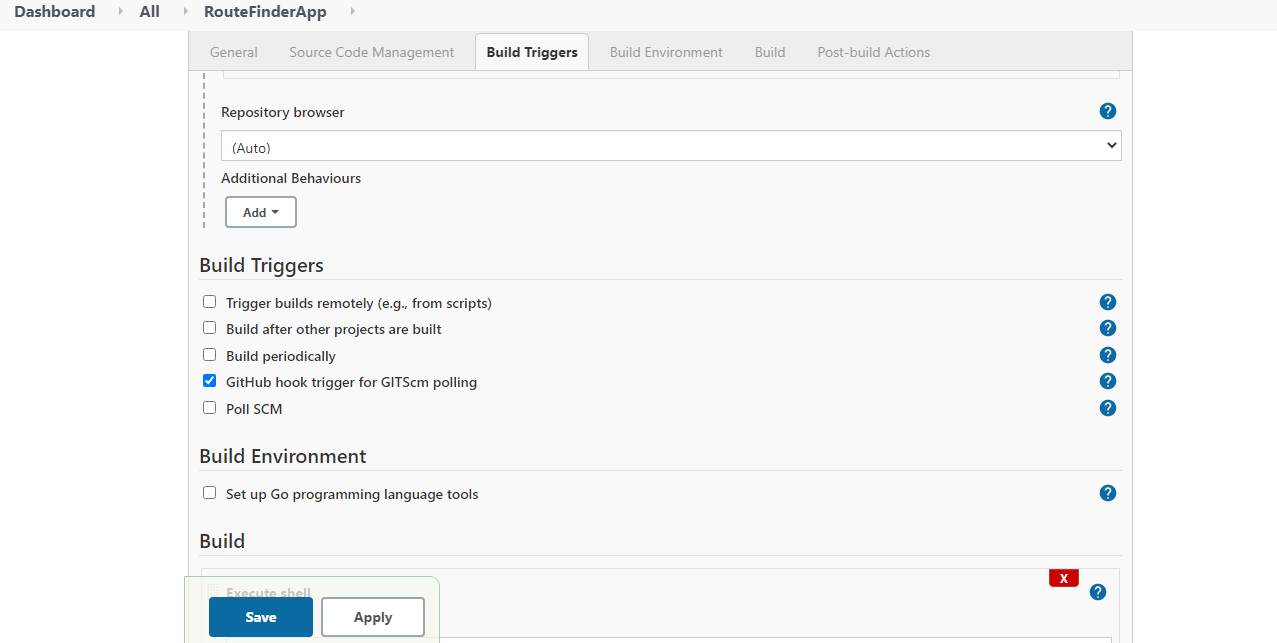
\includegraphics[width=15cm]{images-aws/46-trigger-jenkins.png}
        \caption{Setup Github hook trigger for GITScm polling}
\end{figure}




~\newpage


\subsection{Test the GitHub Webhook}


From \textbf{VSCode}, where we have the project open, we push a new commit to GitHub in order to test the Webhook.


\begin{figure}[H]
    \centering
        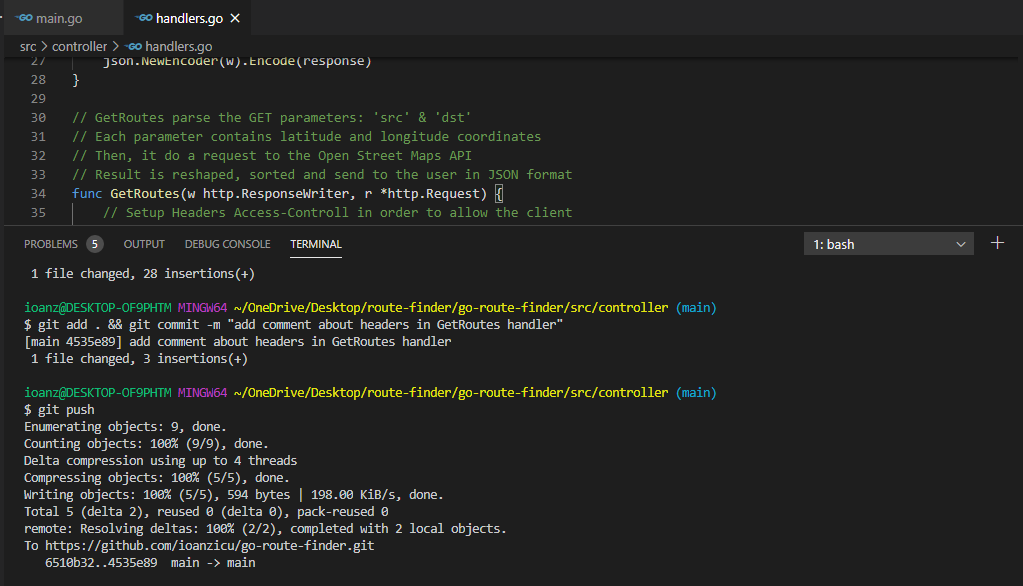
\includegraphics[width=15cm]{images-aws/47-small-commit-after-fixed-branches.png}
        \caption{Commit and Push a new Commit}
\end{figure}


After pushing, we refresh the web page of the project repository on \textbf{GitHub}. In the \textbf{Settings - Webhooks} section we see that the Webhook was activated.


\begin{figure}[H]
    \centering
        \includegraphics[width=15cm]{images-aws/48-successfull-push-webhook.png}
        \caption{Github hook is activated}
\end{figure}


In the Jenkins \textbf{Dashboard} we see that the \textbf{Last Success} build was done 1 minute 45 seconds ago.


\begin{figure}[h!]
    \centering
        \includegraphics[width=15cm]{images-aws/49-triggered-push.png}
        \caption{Project status build - Last Success 1 minute 45 seconds ago}
\end{figure}


From \textbf{Dashboard} we click to the project name and then build number. We can see that the build passed and it was triggered by our \textbf{Push} event.

\begin{figure}[H]
    \centering
        \includegraphics[width=15cm]{images-aws/50-triggered-push-logs.png}
        \caption{Build Logs from the Console Output}
\end{figure}





\subsection{Setup Email Notification at each Build}


In this subsection we will describe how we configured Jenkins to get email notifications for both fail and success build statuses.


First step is to setup \textbf{E-mail Notifications}, for this we go to \textbf{Manage Jenkins} - \textbf{Configure System} and scroll down to \textbf{E-mail Notification} subsection.


We set \textbf{SMTP server} to \textbf{smtp.gmail.com} and click on \textbf{Advanced} button.


The \textbf{Advanced} menu, we:


\begin{itemize}
	\item  select option \textbf{Use SMTP Authentication},
	\item \textbf{User Name} - add Gmail that we created specifically for this purpose,
	\item \textbf{Password} - enter password of Gmail from previous field,
	\item  select option \textbf{Use SSL},
	\item \textbf{SMPT Port} - set to \textbf{465},
	\item \textbf{Reply to Address} - we enter again the same email from the \textbf{User Name} field.
\end{itemize}


\begin{figure}[H]
    \centering
        \includegraphics[width=15cm]{images-aws/51-email-settings.png}
        \caption{Email Notification Configurations}
\end{figure}


Next, we have an option to test the configurations that we setup. But because of the Gmail security policy, we will receive the following error message: \textbf{403 No valid crumb was included in the request.}


This Issue is well known in Jenkins community, so in order to solve it we have to configure \textbf{Compatibility mode for proxy}. 


From Jenkins home page we go to \textbf{Configure Global Security} settings, scroll to \textbf{CSRF Protection} subsection and enable option \textbf{Enable proxy compatibility}. The we click on \textbf{Save} button and go back to \textbf{Email Notification} settings.


\begin{figure}[H]
    \centering
        \includegraphics[width=15cm]{images-aws/52-enable-proxy-compatibility.png}
        \caption{Enable proxy compatibility}
\end{figure}


Now we click the \textbf{Test Configuration} button and make sure that an email was sent successfully. Then we click \textbf{Save} button and go back to Jenkins home page.


\begin{figure}[H]
    \centering
        \includegraphics[width=15cm]{images-aws/53-email-test-configuration.png}
        \caption{Test Configurations for Email Notification}
\end{figure}


Here we can see received test email sent from Jenkins.


\begin{figure}[H]
    \centering
        \includegraphics[width=15cm]{images-aws/54-email-test-confirmation.png}
        \caption{Received Test Email}
\end{figure}


Now we select \textbf{RouteFinderApp} Job, open \textbf{Configure} menu, click on tab \textbf{Build} and from the \textbf{Add post-buidl actions} select \textbf{E-mail Notifications}


\begin{figure}[H]
    \centering
        \includegraphics[width=15cm]{images-aws/55-email-notification-buil-setting.png}
        \caption{Select E-mail Notification from Add post-build actions dropdown}
\end{figure}


In a new window we enter in \textbf{Recipients} field the list of emails separated by whitespace. and enable options \textbf{Send e-mail for every unstable build} and \textbf{Send separate e-mails to individuals who broke the build}.
The recipients will receive email notification at each build.


\begin{figure}[H]
    \centering
        \includegraphics[width=15cm]{images-aws/56-email-notification-post-build-action.png}
        \caption{Add Recipients for Post-build Actions}
\end{figure}




~\newpage


\subsection{Test Email Notification}


To test email notifications we trigger a build and open \textbf{Console Output} window. From the logs we can see the record for sending email to the list of recipients that we have configured in the previous section.


\begin{figure}[H]
    \centering
        \includegraphics[width=15cm]{images-aws/57-email-notification-trigger-build.png}
        \caption{Logs from the Job Build}
\end{figure}


Then we open the Gmail and check for notification email from Jenkins. 
In the figure below we can see how notification email looks. It contains a link to the Jenkins build.


\begin{figure}[H]
    \centering
        \includegraphics[width=15cm]{images-aws/58-gmail-notification-received-full.png}
        \caption{Received Notification Email from Jenkins}
\end{figure}


By clicking on provided URL link in the email, we open specific build webpage in the Jenkins.


\begin{figure}[H]
    \centering
        \includegraphics[width=15cm]{images-aws/59-gmail-notification-link-open.png}
        \caption{Jenkins Build Page that we found in the Email Notification}
\end{figure}






~\newpage


\section{Conclusions}

Jenkins is a powerful open-source tool that allows CI/CD integration for better and faster software development life-cycle. It has a variety of plugins and many ways to customize the build environment. Jenkins jobs can be easily configured and triggered by specific events. 

Integration of Jenkins with GitHub allows us to trigger build at each Push or Pull Request, ensuring that a new feature or modification of the existing code runs properly and passes all the tests. 

In case if build fails, then developers receive feedback about the causes. By doing so the final product is cleaned from the bugs and we can be sure that it will not encounter unexpected errors in production deployment.


~\newpage


\begin{thebibliography}{100}

% CI / CD
	\bibitem{ELEMENTS-CI/CD} \url{https://semaphoreci.com/blog/cicd-pipeline#:~:text=What\%20is\%20a\%20CI\%2FCD,and\%20enable\%20fast\%20product\%20iterations.}	

% Jenkins
	\bibitem{} \url{https://www.jenkins.io/}
	\bibitem{} \url{https://www.tutorialspoint.com/jenkins/index.htm}
	\bibitem{JENKINS-FLOWCHART} \url{https://www.tutorialspoint.com/jenkins/jenkins_overview.htm}
	\bibitem{} \url{https://en.wikipedia.org/wiki/Jenkins_(software)}

% GitHub
	\bibitem{} \url{https://en.wikipedia.org/wiki/GitHub}

% AWS
	\bibitem{} \url{chrome-extension://oemmndcbldboiebfnladdacbdfmadadm/https://d1.awsstatic.com/Projects/P5505030/aws-project_Jenkins-build-server.pdf}
	\bibitem{JENKINS-BUILD-SERVER} \url{https://aws.amazon.com/getting-started/hands-on/setup-jenkins-build-server/}

% Go Jenkins
	\bibitem{} \url{https://bmuschko.com/blog/go-on-jenkins/#:~:text=Jenkins}

% Pull Request
	\bibitem{} \url{https://devopscube.com/jenkins-build-trigger-github-pull-request/}


	\bibitem{} \url{https://www.blazemeter.com/blog/how-to-integrate-your-github-repository-to-your-jenkins-project}

% Email Build Notification
	\bibitem{} \url{https://medium.com/@arun.dev/get-email-notification-for-jenkins-build-failure-and-success-d59154dc639a}

\end{thebibliography}



\end{document}